%%%%%%%%%%%%%%%%%%%%%%%%%%%%%%%%%%%%%%%%%
% Masters/Doctoral Thesis
% LaTeX Template
% Version 2.5 (27/8/17)
%
% This template was downloaded from:
% http://www.LaTeXTemplates.com
%
% Version 2.x major modifications by:
% Vel (vel@latextemplates.com)
%
% This template is based on a template by:
% Steve Gunn (http://users.ecs.soton.ac.uk/srg/softwaretools/document/templates/)
% Sunil Patel (http://www.sunilpatel.co.uk/thesis-template/)
%
% Template license:
% CC BY-NC-SA 3.0 (http://creativecommons.org/licenses/by-nc-sa/3.0/)
%
%%%%%%%%%%%%%%%%%%%%%%%%%%%%%%%%%%%%%%%%%

%----------------------------------------------------------------------------------------
%	PACKAGES AND OTHER DOCUMENT CONFIGURATIONS
%----------------------------------------------------------------------------------------
%\UseRawInputEncoding
%\DeclareUnicodeCharacter{00A0}{~}
\documentclass[ 
11pt, % The default document font size, options: 10pt, 11pt, 12pt
%oneside, % Two side (alternating margins) for binding by default, uncomment to switch to one side
french, % ngerman for German
singlespacing, % Single line spacing, alternatives: onehalfspacing or doublespacing
% draft, % Uncomment to enable draft mode (no pictures, no links, overfull hboxes indicated)
%nolistspacing, % If the document is onehalfspacing or doublespacing, uncomment this to set spacing in lists to single
% liststotoc, % Uncomment to add the list of figures/tables/etc to the table of contents
%toctotoc, % Uncomment to add the main table of contents to the table of contents
parskip, % Uncomment to add space between paragraphs
%nohyperref, % Uncomment to not load the hyperref package
headsepline, % Uncomment to get a line under the header
%chapterinoneline, % Uncomment to place the chapter title next to the number on one line
%consistentlayout, % Uncomment to change the layout of the declaration, abstract and acknowledgements pages to match the default layout
openany, %% Use this option to make chapters start on the next page, irrespective of whether it's an odd or even numbered page
]{MastersDoctoralThesis} % The class file specifying the document structure

\usepackage{mathpazo} % Use the Palatino font by default
% \usepackage[light,condensed,math]{iwona}  %% Comment above and uncomment this to use the Iwona font

% \setcounter{tocdepth}{4} %% Use this to set numbering depth for sections in the toc (already set in the Class)
\setcounter{secnumdepth}{3} %% Use this to set numbering depth for sections in the whole document

\graphicspath{ {./Figures/} } %% To load all images in this document from the Figures directory
\DeclareGraphicsExtensions{.pdf,.png}  %% Use to this to set the priority for extensions leading
\usepackage{subcaption} %% Use to make subgraphics
\usepackage{float} %% Use this to control where the images are placed compared to thier related text

\usepackage{amsmath,bm,mathtools} %% Use this to include the "align" environment in witch equations can be made easier
\usepackage{physics} %% To have physical terms like the divergence operator
\newcommand{\bvec}[1]{\mathbf{#1}}  %% Use this for make you vectors look bolded

\usepackage[backend=bibtex,style=authoryear,maxnames=2,natbib=true]{biblatex} % Use the bibtex backend with the authoryear citation style (which resembles APA)

\addbibresource{bibliographie.bib} % The filename of the bibliography

\usepackage[autostyle=true]{csquotes} % Required to generate language-dependent quotes in the bibliography 

%----------------------------------------------------------------------------------------
%	MARGIN SETTINGS
%----------------------------------------------------------------------------------------

\geometry{
	paper=a4paper, % Change to letterpaper for US letter
	inner=0.75in, % Inner margin
	outer=0.75in, % Outer margin
	bindingoffset=.5cm, % Binding offset
	top=1.5cm, % Top margin
	bottom=1.5cm, % Bottom margin
	%showframe, % Uncomment to show how the type block is set on the page
}

%----------------------------------------------------------------------------------------
%	THESIS INFORMATION
%----------------------------------------------------------------------------------------

\thesistitle{Modélisation 2D de l’équation du transfert radiatif et reconstruction de la densité par un réseau de neurones} % Your thesis title, ths is used in the title and abstract, print it elsewhere with \ttitle
\supervisor{Emmanuel \textsc{Franck} \\ Laurent \textsc{Navoret} \\ Vincent \textsc{Vigon}} % Your supervisor's name, this is used in the title page, print it elsewhere with \supname
\examiner{Christophe \textsc{PRUD'HOMME}} % Your examiner's name, this is not currently used anywhere in the template, print it elsewhere with \examname
\degree{Master CSMI} % Your degree name, this is used in the title page and abstract, print it elsewhere with \degreename
\author{Roussel Desmond \textsc{Nzoyem}} % Your name, this is used in the title page and abstract, print it elsewhere with \authorname
\addresses{} % Your address, this is not currently used anywhere in the template, print it elsewhere with \addressname

\subject{Mathématiques appliquées} % Your subject area, this is not currently used anywhere in the template, print it elsewhere with \subjectname
\keywords{} % Keywords for your thesis, this is not currently used anywhere in the template, print it elsewhere with \keywordnames
\university{\href{http://www.unistra.fr}{Université de Strasbourg}} % Your university's name and URL, this is used in the title page and abstract, print it elsewhere with \univname
\department{\href{https://mathinfo.unistra.fr/}{UFR de mathématiques et d'informatique}} % Your department's name and URL, this is used in the title page and abstract, print it elsewhere with \deptname
\group{\href{http://irma.math.unistra.fr/rubrique162.html}{équipe MOCO}} % Your research group's name and URL, this is used in the title page, print it elsewhere with \groupname
\faculty{\href{https://mathinfo.unistra.fr/}{UFR de mathématiques et d'informatique}} % Your faculty's name and URL, this is used in the title page and abstract, print it elsewhere with \facname

\AtBeginDocument{
\hypersetup{pdftitle=\ttitle} % Set the PDF's title to your title
\hypersetup{pdfauthor=\authorname} % Set the PDF's author to your name
\hypersetup{pdfkeywords=\keywordnames} % Set the PDF's keywords to your keywords
}

\begin{document}

\frontmatter % Use roman page numbering style (i, ii, iii, iv...) for the pre-content pages

\pagestyle{plain} % Default to the plain heading style until the thesis style is called for the body content

%----------------------------------------------------------------------------------------
%	TITLE PAGE
%----------------------------------------------------------------------------------------

\begin{titlepage}

\begin{figure}[!htb]
   \begin{minipage}{0.40\textwidth}
     \centering
     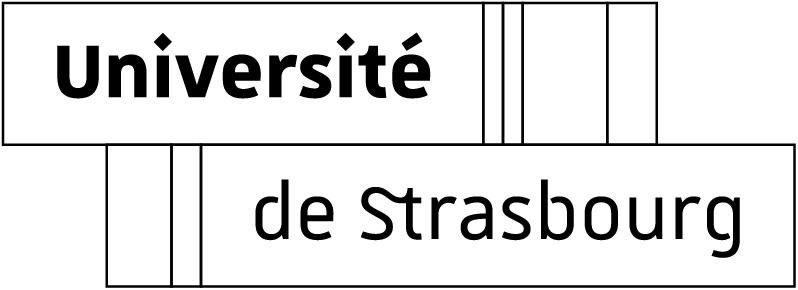
\includegraphics[width=.7\linewidth]{LogoUnistra}
     \label{Fig:LogoUnistra}
   \end{minipage}\hfill
   \begin{minipage}{0.30\textwidth}
     \centering
     
\includegraphics[width=.7\linewidth]{LogoIRMA}
     \label{Fig:LogoIRMA}
   \end{minipage}
\end{figure}


\begin{center}

\vspace*{.06\textheight}
% {\scshape\LARGE \univname\par}\vspace{1.5cm} % University name
\textsc{\Large Rapport de stage}\\[0.5cm] % Thesis type

\HRule \\[0.4cm] % Horizontal line
{\huge \bfseries \ttitle\par}\vspace{0.4cm} % Thesis title
\HRule \\[1.5cm] % Horizontal line

\begin{minipage}[t]{0.4\textwidth}
\begin{flushleft} \large
\vspace{7mm}
\emph{Auteur}\\
\href{http://www.johnsmith.com}{\authorname} % Author name - remove the \href bracket to remove the link
\end{flushleft}
\end{minipage}
\begin{minipage}[t]{0.4\textwidth}
\begin{flushright} \large
\emph{Maitres de stage} \\
\href{http://www.jamessmith.com}{\supname} % Supervisor names - remove the \href bracket to remove the link
\\ \vspace{5mm}
\emph{Enseignant référent} \\
\href{http://www.jamessmith.com}{\examname} % Examiner's name - remove the \href bracket to remove the link
\end{flushright}
\end{minipage}\\[2cm]

% \vfill

\large \textit{Stage réalisé dans le cadre du \degreename}\\[0.2cm] % University requirement text
\textit{du 15 juin 2020 au 15 août 2020}\\[0.2cm]
\textit{à l'initiative de l'\groupname}\\[0.2cm] % Research group
\textit{au sein de l'\deptname}\\[2cm] % Department name

\large Année académique 2019 - 2020

\vfill

{\large \today}\\[4cm] % Today's date
% 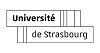
\includegraphics{Logo_UNIV} % University/department logo - uncomment to place it

% \vfill
\end{center}
\end{titlepage}

%----------------------------------------------------------------------------------------
%	DECLARATION PAGE
%----------------------------------------------------------------------------------------
%
% \begin{declaration}  
% \addchaptertocentry{\authorshipname} % Add the declaration to the table of contents
% \noindent I, \authorname, declare that this thesis titled, \enquote{\ttitle} and the work presented in it are my own. I confirm that:
%
% \begin{itemize}
% \item This work was done wholly or mainly while in candidature for a research degree at this University.
% \item Where any part of this thesis has previously been submitted for a degree or any other qualification at this University or any other institution, this has been clearly stated.
% \item Where I have consulted the published work of others, this is always clearly attributed.
% \item Where I have quoted from the work of others, the source is always given. With the exception of such quotations, this thesis is entirely my own work.
% \item I have acknowledged all main sources of help.
% \item Where the thesis is based on work done by myself jointly with others, I have made clear exactly what was done by others and what I have contributed myself.\\
% \end{itemize}
%
% \noindent Signed:\\
% \rule[0.5em]{25em}{0.5pt} % This prints a line for the signature
%
% \noindent Date:\\
% \rule[0.5em]{25em}{0.5pt} % This prints a line to write the date
% \end{declaration}
%
% \cleardoublepage

%----------------------------------------------------------------------------------------
%	QUOTATION PAGE
%----------------------------------------------------------------------------------------
%
% \vspace*{0.2\textheight}
%
% \noindent\enquote{\itshape Thanks to my solid academic training, today I can write hundreds of words on virtually any topic without possessing a shred of information, which is how I got a good job in journalism.}\bigbreak
%
% \hfill Dave Barry

%----------------------------------------------------------------------------------------
%	ABSTRACT PAGE
%----------------------------------------------------------------------------------------
%
% \begin{abstract}
% \addchaptertocentry{\abstractname} % Add the abstract to the table of contents
% The Thesis Abstract is written here (and usually kept to just this page). The page is kept centered vertically so can expand into the blank space above the title too\ldots
% \end{abstract}

%----------------------------------------------------------------------------------------
%	ACKNOWLEDGEMENTS
%----------------------------------------------------------------------------------------

\begin{acknowledgements}
\addchaptertocentry{\acknowledgementname} % Add the acknowledgements to the table of contents
\qquad Je tiens à remercier dans un premier temps mes maîtres de stages MM. Emmanuel \textsc{Franck}, Laurent \textsc{Navoret}, et Vincent \textsc{Vigon} de m’avoir permis d’effectuer un stage scientifique très enrichissant dans les meilleurs conditions possibles, compte tenu de la situation sanitaires liée au COVID-19.

Je remercie aussi mes camarades de CSMI Guillaume \textsc{Steimer} et Léo \textsc{Bois} pour leurs conseils qui ont été instrumental dans l'amélioration de mes résultats.
\end{acknowledgements}

%----------------------------------------------------------------------------------------
%	LIST OF CONTENTS/FIGURES/TABLES PAGES
%----------------------------------------------------------------------------------------

\tableofcontents % Prints the main table of contents

% \listoffigures % Prints the list of figures

% \listoftables % Prints the list of tables

%----------------------------------------------------------------------------------------
%	ABBREVIATIONS
%----------------------------------------------------------------------------------------

% \begin{abbreviations}{11} % Include a list of abbreviations (a table of two columns)
% 
% \addchaptertocentry{\abbreviations} % Add the abbreviations to the table of contents
% \textbf{ETR} & \textbf{E}quation (du) \textbf{T}ransfert \textbf{R}adiatif\\
% \textbf{ETL} & \textbf{E}quilibre \textbf{T}hermique \textbf{L}ocal\\
% \textbf{UFR} & \textbf{U}nite de\textbf{F}ormation et de \textbf{R}echerche de l'Universite de Strasbourg
% 
% \end{abbreviations}

%----------------------------------------------------------------------------------------
%	PHYSICAL CONSTANTS/OTHER DEFINITIONS
%----------------------------------------------------------------------------------------

% \begin{constants}{lr@{${}={}$}l} % The list of physical constants is a three column table
% 
% The \SI{}{} command is provided by the siunitx package, see its documentation for instructions on how to use it
% 
% Speed of Light & $c_{0}$ & \SI{2.99792458e8}{\meter\per\second} (exact)\\
% Constant Name & $Symbol$ & $Constant Value$ with units\\

% \end{constants}

%----------------------------------------------------------------------------------------
%	SYMBOLS
%----------------------------------------------------------------------------------------

\begin{symbols}{rcc} % Include a list of Symbols (a three column table)
\label{sec:symbols}
\textbf{Symbole} & \textbf{Définition} & \textbf{Unité} \\
\addlinespace % Gap to separate the Roman symbols from the Greek

$x$ & Abscisse & \si{\m} \\
$y$ & Ordonnée & \si{\m} \\
$\bm{x}$ & Vecteur position & \si{\m} \\
$\bm{\Omega}$ & Vecteur direction de propagation des photons & \si{\m^2 \per \m^2} \\
$\nu$ & Fréquence & \si{Hz} \\
$p$ & Fonction de distribution angulaire de « scattering » &  \\
$I$ & Intensité spécifique de radiation & \si{W \per m^2 \per sr  \per Hz} \\
$B$ & Fonction de Planck & \si{W \per m^2 \per sr  \per Hz} \\

\addlinespace % Gap with real SI dimensions

$\rho$ & Densité du milieu & \si{\g\per\cm\cubed} \\
$\sigma_a$ & Opacité d'absorption & \si{\per\cm} \\
$\sigma_c$ & Opacité de dispersion (de « scattering ») & \si{\per\cm} \\

\addlinespace % Gap to separate inputs

$t$ & Temps & \si{sh} \\
$C_v$ & Capacité thermique du milieu & \si{Jerk \per\g \per keV} \\
$a$ & Constante de radiation ($E = aT^4$)& \si{g \per cm \per sh^2  \per keV } \\
$c$ & Vitesse de la lumière & \si{\cm \per sh} \\

\addlinespace % Gap to separate output

$T$ & Température matière & \si{keV} \\
$E$ & Energie des photons & \si{g \per \cm \per sh^2} \\
$F$ & Flux de photons & \si{g \per sh^2} \\

\end{symbols}

%----------------------------------------------------------------------------------------
%	DEDICATION
%----------------------------------------------------------------------------------------

% \dedicatory{For/Dedicated to/To my\ldots}

%----------------------------------------------------------------------------------------
%	THESIS CONTENT - CHAPTERS
%----------------------------------------------------------------------------------------

\mainmatter % Begin numeric (1,2,3...) page numbering
\setlength{\parindent}{5ex} %% Set the paragraph indentation as from this line

\pagestyle{thesis} % Return the page headers back to the "thesis" style

% Include the chapters of the thesis as separate files from the Chapters folder
% Uncomment the lines as you write the chapters

% Chapter 1

\chapter{Introduction} % Main chapter title

\label{Chapter1} % For referencing the chapter elsewhere, use \ref{Chapter1} 

%----------------------------------------------------------------------------------------

% Define some commands to keep the formatting separated from the content 
\newcommand{\keyword}[1]{\textbf{#1}}
\newcommand{\tabhead}[1]{\textbf{#1}}
\newcommand{\code}[1]{\texttt{#1}}
\newcommand{\file}[1]{\texttt{\bfseries#1}}
\newcommand{\option}[1]{\texttt{\itshape#1}}

%----------------------------------------------------------------------------------------

En 2015, le réseau de neurones vainqueur de l'ILSVRC \footnote{ImageNet Large Scale Visual Recognition Challenge} obtient une précision de 97.3 \% ce qui conduit les chercheurs à postuler que les machines peuvent identifier les objets dans des images mieux que les humains \parencite{Reference1}. Depuis lors, le domaine du Machine Learning a continué à prendre de l'ampleur. Aujourd'hui ses applications se multiplient dans plusieurs secteurs d'activité parmi lesquelles l'automobile, la finance, le divertissement, et plus important, celui de la santé à travers l'imagerie médicale.

Les tumeurs ont des propriétés de propagation différentes des tissus qui les entourent \footnote{Les tissus cancéreux sont généralement plus denses que les tissus sains.}. Étant donné un domaine avec une onde qui s'y propage, reconstruire sa densité à l'aide du signal temporel mesuré sur ses bords constitue un problème inverse. Les problèmes inverses sont très importants en sciences mathématiques et ont des applications variées en imagerie médicale, radar, vision, etc. Ils sont malheureusement très difficiles à résoudre car ils nécessitent l'utilisation d'algorithme d'optimisation avancés. Les réseaux de neurones artificiels se présente comme une méthode potentiellement moins couteuse mais plus rapide.

Grace à son unité mixte de recherche IRMA, l'UFR de mathématique et d'informatique de l'Université de Strasbourg est un pôle de recherche en mathématiques appliquées. À travers ses équipes MOCO et Probabilités, l'IRMA s'intéresse aux problématiques de modélisation des EDP et de Machine Learning, raison pour laquelle j'ai choisi d'y effectuer mon stage de master 1 CSMI\footnote{Calcul Scientifique et Mathématiques de l'Information}. Au cours de ce stage (du 15 juin au 15 août 2020), j'ai pu m'intéresser au problème inverse de reconstruction de la densité d'un domaine par un réseau de neurones convolutif (CNN).

Ce stage a été suivi par les enseignants-chercheurs MM. Emmanuel \textsc{Franck}, Laurent \textsc{Navoret}, et Vincent \textsc{Vigon} et s'inscrit dans la continuation d'un projet (encadré par la même équipe) qui s'est déroulé du 19 mars au 28 mai 2020. Le projet consistait en la simulation 1D d'un schéma de « splitting » pour le modèle P1 de l'équation du transfert radiatif couplé avec la matière. Le stage quant à lui a essentiellement consisté en la simulation du même schéma en 2D, et en la reconstruction de la densité par un CNN. Plus généralement, ce stage a été l'opportunité pour moi d'apprendre sur les EDP et l'apprentissage profond tout en me familiarisant avec l'interface de programmation de la librairie de réseaux de neurones Keras. 

En vue de rendre compte de manière fidèle des deux mois passés au sein de l'IRMA, il apparait logique de présenter en titre de préambule le cadre du stage et son environnement technique. Ensuite il s'agira de présenter les différentes missions et tâches qui j'ai pu effectuer. Enfin je présenterais un bilan du stage, en incluant les différents apports et enseignements que j'ai pu en tirer.

% Chapter 2

\chapter{Présentation de l'IRMA} % 2 nd chapter title

\label{Chapter2} % For referencing the chapter elsewhere, use \ref{Chapter2} 

\textit{Les informations presentes dans cette section sont entierement issues du \href{http://irma.math.unistra.fr/}{site web de l'IRMA}}

Cree en 1966 par Jean Frenjel et Gearges Reeeb, l'IRMA\footnote{Institut de Recherche Mathématique Avancée} est une  unité mixte de recherche (UMR 7501) sous la double tutelle du CNRS (a travers l'INSMI\footnote{Institut National des Sciences Mathématiques et de leurs Interactions}) et de l’Université de Strasbourg (UFR de Mathématique et d’Informatique).

Dirigee par le professeur Philippe Helluy, l'IRMA comporte environ 130 membres. On y compte enviro 87 chercheurs et enseignants-chercheurs permanent et une qurantaine de non permanents repartis en 8 equipes de recherche.

Les activites majeures de l'organisme sont l'organisation des seminaires, des journees, des colloques et des conferences. Ces activites sont renforcees par les nombreux partenariats qu'elle maintient dans les secteurs academique(Cemosis, Labex IRMIA, etc..) et indutriel (AxesSIM, Electis, etc..).

%----------------------------------------------------------------------------------------

\section{Structure de l'organisation}
L'organigramme de l'entreprise representant ses sections majeures est donne a la figure \ref{fig:OrganigrammeIRMA}).

\begin{figure}[!h]
\centering
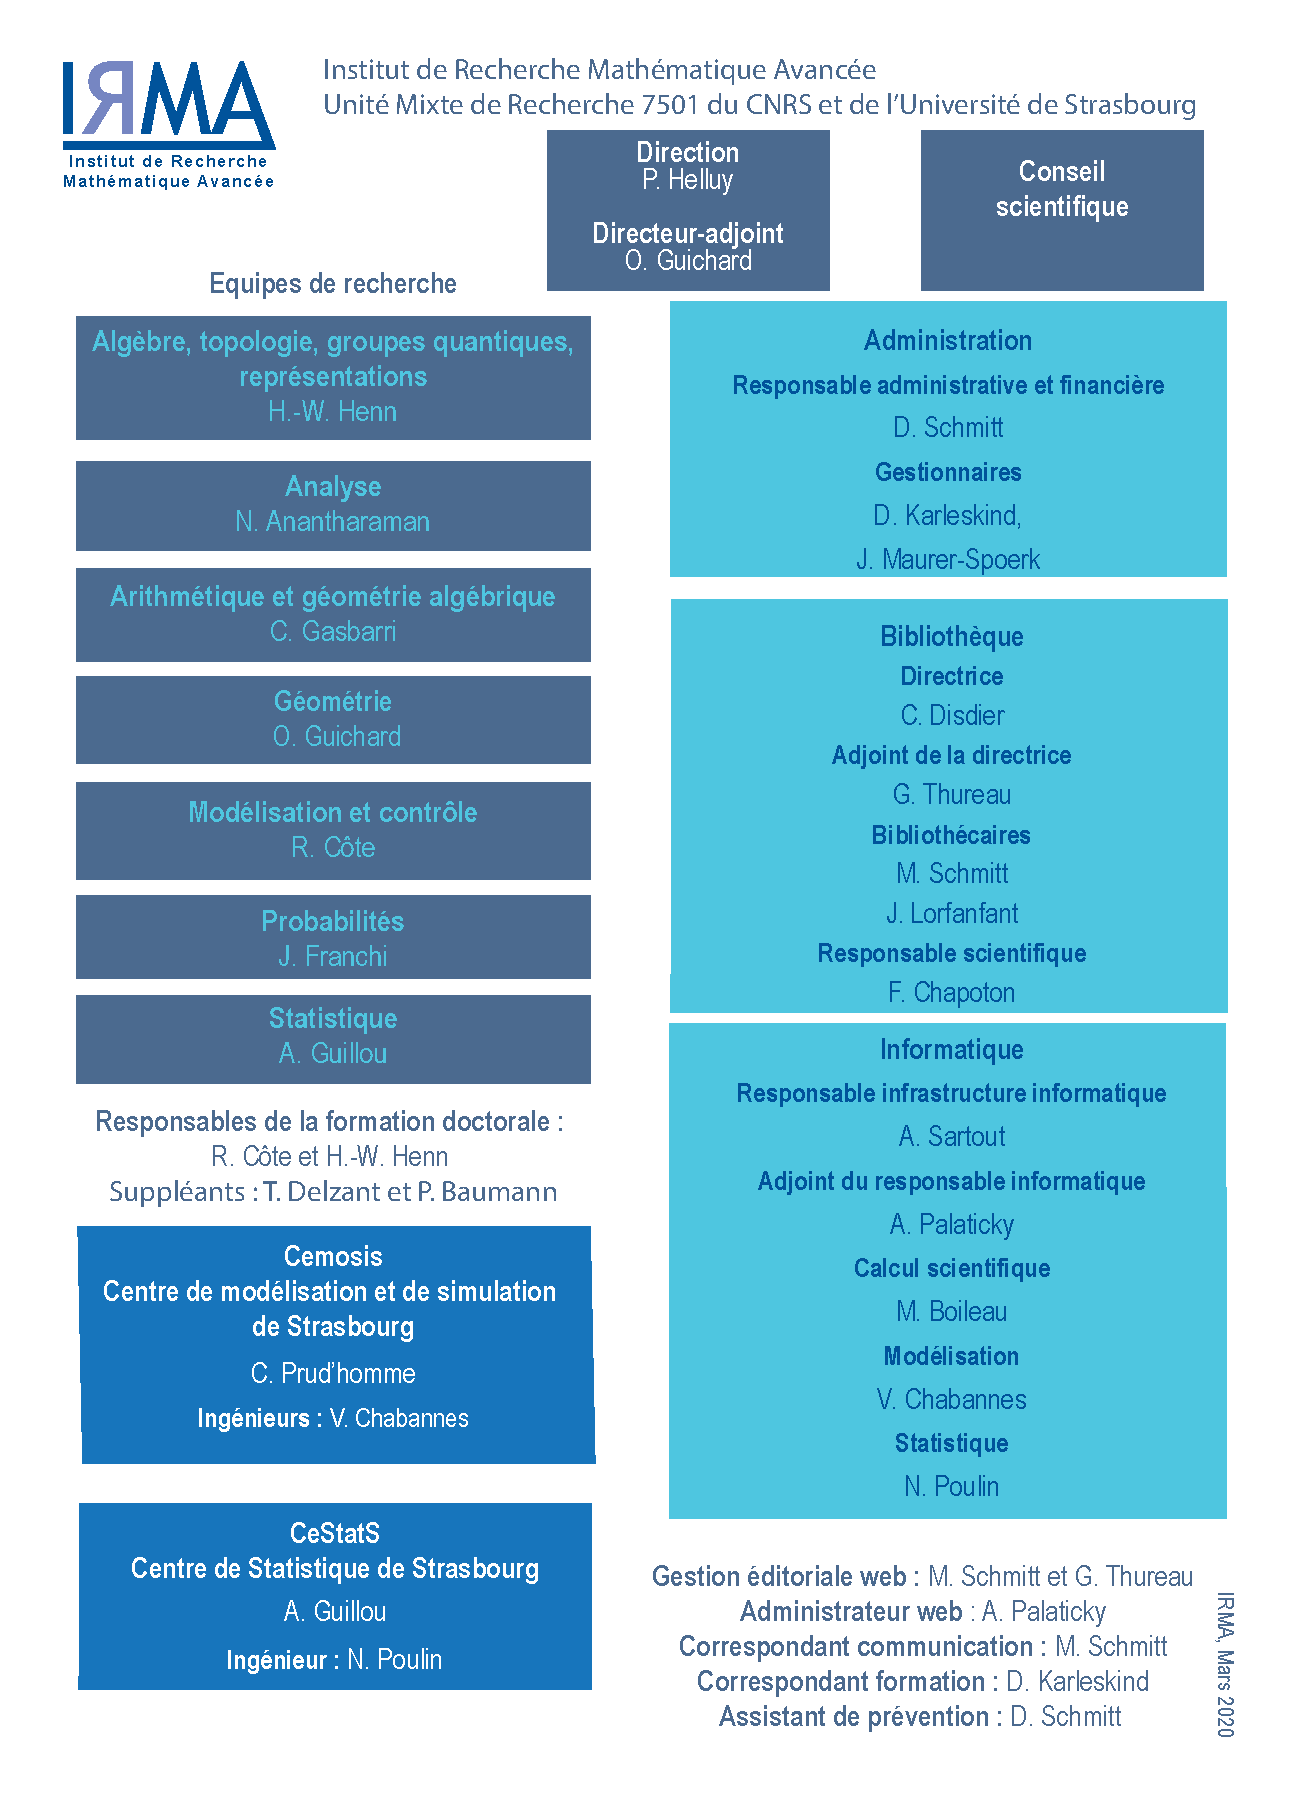
\includegraphics[width=.8\linewidth]{OrganigrammeIRMA} 
\decoRule
\caption[Organigramme de l'IRMA]{Organigramme representant l'organisaiton de l'IRMA au mois de mars 2020 \parencite{Reference7}}
\label{fig:OrganigrammeIRMA}
\end{figure}

%----------------------------------------------------------------------------------------

\section{Les équipes MOCO et Probabilite}

L'equipe MOCO \footnote{MOdelisation et COntrole} se compose de specilistes des EDP, de la theorie deu controle, ddu calcul scientifique et haute performance et des statistiques. Ses activites s'etendent a l'internationale et dans l'indutriel (REF, ...). Les enseignants-chercehurs MM. Emmanuel Franck et en Laurent Navoret y sont responsables des seminaires en equations aux derivees partielles. 

L'equipe probabilite est composee d'experts en calcul de probabilite. Ses membres se retrouvent regulierement lors du "seminaire stochatique". A cette equipe apartient M. Vincent Vigon. 

Je tiens une fois de plus a remercier les trois chercheurs mentiones ci-hauts qui ont encadrer ce stage. La combinaison de ces deux equipes dont ils font partie a permis de faire face aux deux aspects de ce stage. Premierement la modelisation d'EDP et finalement l'utilisation des reseaux de neurones.

%----------------------------------------------------------------------------------------

% Chapter 3

\chapter{Modelisation de l'EDP en 2D} % 3rd chapter title

\label{Chapter3} % For referencing the chapter elsewhere, use \ref{Chapter3} 

%----------------------------------------------------------------------------------------

Ayant resolu le modele en 1D durant le stage, on procede dans cette partie a sa modelisation en 2D. Il s'agit de resoudre le probleme direct du transfer radiatif avant de passer au probleme inverse dans la partie suivante. On rappelle breivement le modele considere avant de decrite l'implementation que utilisee.

\section{Le transfert radiatif}


On considère un rayonnement transporté par des particules de masse nulle appelés photons. Lorsqu'ils se touvent en presence de la matiere, les photons inteassgissent avec celle. Trois phonomees sont preponderant (\ref{Fig:TranfertRadiatif}):

\begin{itemize}
 \item l'emission: Les photons sont emis en reponse aux electrons excites descendants a des niveaux d'energie plus bas. Ce phenomenes est caraterise par l'opacite d'émission $\sigma_e$. Il s'agit de l'inverse du libre parcours d'emision \footnote{Le libre par cours moyen d'emission represente la distance moyenne entre deux emissions de photons. Les libres parcours d'absorption et de dispersion sont definis de maniere similaire}. Plus la temperature matiere est elevee, plus ce phenomene est important.
 \item l'absorption: A l'inverse, certains photons sont absorbes par la matiere. Ce pehenomene se caraterise par l'opacite d'absorption $\sigma_a$. Lorsqu'on est a l'equilibre thermique, $\sigma_e = \sigma_e$.
 \item la dispersion (ou "scaterring" ou parfois diffusion): Certains photons sont devies de leur trajectoire par la matiere. Ce phenomme se caraterise non seulement par son opacite de scatering $\sigma_c$ \footnote{ $\sigma_a$ et $\sigma_c$ sont definis de maniere similaire a $\sigma_e$}, mais aussi par une fonction de distribution angulaire decrivant la maniere dont les photons sont devies.
\end{itemize}

(IMAGE DU TRANFER RADIATIF)

L'equation du transfer radiatif (1) represente un bilan d'energie lie au rayonnement au niveau microscopique. Nous nous placerons dans le cas particulier d'equilibre thermodynamique local (ETL)\footnote{etat dans lequel on peut definir une temperature pour chaque point du domaine, et l'emission est decrite par la fonction de Planck \parencite{Reference3}}. L'equilibre radiatif \footnote{il se produit si la matiere est a l'equilibre avec le reyonnement. Si on est dans l'ETL, les photons sont emis suivant la fonction de Planck a la temperature de la matiere} quant a lui sera considere comme condition initiale pour les simulations.

(EQUATION 1) - ETR (et definition des termes)

Il est possible de modeliser l'ETR a travers plusieurs modeles. Le modele P1 est un modele macroscopique \footnote{ils ne prennent en compte que les varaibles d'espace et de temps et spm obtenu par integration des termes microscopique tels que I par rapport a la frequence et la direction} aux moments (d'ordre 2), lineaire et hyperbolique. Vu que l'energie du rayonnement n'est pas convervee durant sont interaction avec la matiere, il faut coupler le modele P1 avec une equation regissant l'energie de la matiere. On utilisera une equation d'energie amtiere simplifiee qui ne tient compte que des termes d'echange avec le rayonnement. Le modele P1 couple a la matiere (REF FRACNK) est presente ci-bas:

(EQUATION 2) - MODELE P1  E, F, et T)

Comme on peut le voir a travers la definition de $E$ et $F$, notre modele est dit "gris" car nous l'integrons sur tout le spectre de frequence. En effet, nous ne nous interressons qu'au rayonnement a travers son bilan d'energie transporte par le flux radiatif. Sur ce point, la version du modele P1 que nous avons utilise est mois precise qu'un modele microscopique base soit sur une methode Monte-Carlo ou une methode des ordonnes discrete. Neanmoins notre modele presente l'avantage d'etre tres peu couteux et relativement facile a implementer \parencite{Reference3}. 
%----------------------------------------------------------------------------------------

\section{Schéma de splitting}

Le modele P1 tend vers une equation de diffusion lorsque les opcites d'absorption ($sigma_a$) et de dispersion ($sigma_c$) sont elevees (de facon a ce que $c/sigma_a = 1$). Les schema classiques tels que le schema de Rusanov ne sont pas assez precis pour capturer cette propriete. 

(EQ 3 - LIMITE DE FISSUSION)

Le schema en 2 etape (ou de Splitting) propose par (franck) est assez precis pour traduire la limite de diffusion. Les deux etapes sont resumees co-bas.


\subsection{Etape 1}
La premiere etape (dite etape de couplage ou d'equilibre, ou etape de relaxation de la temperature) permet de regler la temperature sur chaque maille (independament des autres mailles). On ne considere que les equations ou la temperature est impiquee (equations 1 et 3 du modele p1), en fixant la valeur du flux sur chaque maille. Il s'agit d'une methode de point fixe qui est toujorus definie. \parencite{Reference2}

Le domaine rectangulaire est suppose discretise en $N \times M$ mailles uniformes. $j$ denote l'identifiant d'une cellule (Figure \ref{fig:2DMesh}).

(SCHEMA DE SPLiTTING - etape 1)

On itere sur q jusq'a ce que E et $\Theta$ convergent vers $E^*$ et $\Theta^*$.

\subsection{Etape 2}
Il s'agit ici de resoudre les deux EDP hyperboliques en 1 et 2. 
Avasnt d'qttquer le schema schema de splitting, on note que les equations 1 et 2 du modele P1 sont hyperboliques et que La methode des volumes finis est donc adaptee pour les resoudre.

(VOLUMES FINIS)

Nous retournons donc sur le maillage disretise en definisant les different flux numeriques impliques. Durant cette etape, il faut considerer l'ajout de mailles fantommes, ce qui porte le nombre total de volumes a $(N+2) \times (M+2)$.

\begin{figure}[H]
\begin{subfigure}{.6\textwidth}
  \centering
  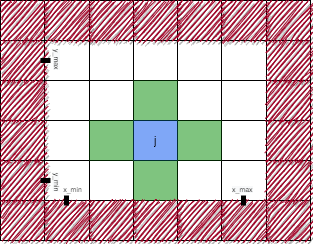
\includegraphics[width=.8\linewidth]{Dicretisation2D}  
  \caption{Dicretisation du domaine}
  \label{fig:Discretisation2D}
\end{subfigure}
\begin{subfigure}{.4\textwidth}
  \centering
  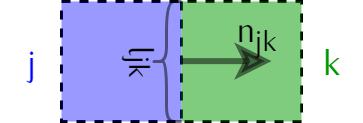
\includegraphics[width=.8\linewidth]{Interaction2D}  
  \caption{Interaction entre deux mailles j et k}
  \label{fig:Interaction2D}
\end{subfigure}
\caption{Dicretisation du maillage 2D. Sur la figure (A), on peut observer les mailles dites "fantomes" hachurees en rouge. Les quatre maille voisine d'une maille j sont indiquees en vert. Le volume de la maille j est definie par $\Omega_j$. Le nombre de mailles suivant l'rizontale $M$ est choisi telle que le maillage soir uniforme i.e $\Delta x = \frac{x_{max}-x_{min}}{N} = \frac{y_{max}-y_{min}}{M} = \Delta y$. Sur la figure (B), on observe la defintion de la normale sortante $n_{jk}$ de la mailles j. On peut aussi observer la longeur caracteristique $l_{jk}$}
\label{fig:2DMesh}
\end{figure}

(SCHEMA DE SPLiTTING etape 2) (\parencite{Reference4})

%----------------------------------------------------------------------------------------

\section{Implementation en C++}

Le dode de calcul a ete develope durant la 4 eme semaine du stage. Etant donne des parametre du probleme, il permet d'exporter les signaux temporels $E, F \text{et} T$ sur les quatres bords du domaine. Pour raisons de visualisation, il permet aussi dd'exporter les signaux sur l'entierete du domaine en tout temps. Ces signaux peuvent ensuite etre visualiser sous forme d'une animation a l'aide d'un notebook construit a cet effet.

L'executable se nomme \verb|transfer| et est disponible avec le reste du code sur le repository Github \href{https://github.com/desmond-rn/projet-inverse-2d}{projet-inverse-2d}.

\subsection{Configuration du modele}

L'executable necessite un fichier de Configuration pour s'excuter. Les parametres a definir sont indiques ci-dessous.

(RAPPELLER L'ASPECT D'UN FICHIER CONFIG)

Un exemple de fichier de configuration pourrait se predenter comme ceci:

(IMAGE DF SIMU)


\subsection{Sauvegarde des données}

Comme mentione ci-haut, on dispose de deux options pour sauvegarder les resultats de la simulation:

\begin{itemize}
 \item sous le forme CSV: Ce mode permet une visualisation facile des resultats a l'aide du noteook. Il est tres couteux en espace memoire et necessite la Librairie Pandas pour le lire en forme de dataframe. Cette operation prend une quantite non negligeagle de RAM, ce qui peut nuire a l'usage qu'on veut faire des donnes.
 
 \item sous le format SDS \footnote{source-densite-signal}: Ce format binaire ne sauvegarde que les informations les plus importante de la simualtion. En locurence la source utilisee, la densite du domaine, et les diffetents signaux sur les bords du domaine. Il est particulieremtnt interressant pour generer les donnees necessaires a l'apprentissage. Les details concernatn la ce format sont donnes en annexe \ref{AppendixA}.
\end{itemize}

%----------------------------------------------------------------------------------------

\section{Résultats}

Queslques resultats obtenus sont presentes ici. Les images ci-bas sont obtenus avec le fichier de configuration (IMAGE DF SIMU). La source est une onde sinusoidale placee en $E$ sur la gauche. La densitee en particulier a la forme d'un signal en crenau egale a 0.1 en dehors du crenau et a 10 en dehors. Les opacites d'absorbes sont proportionelles a la densite.

(ENERGIE ET FLUX OBSTACLE CIRCULAIRE - au temps final)

On peut observer une asorption presque totale du signal au niveau du crenau du a la forte valeur des opacite d'absorption et d'emission. En ce sens, le saut de densite agit comme un obstacle a la propagation du signal. l'evolution de l'energie et du flux sur les bords du domaine traduit l'effet qu'a la densite sur la propagation du signal. Sur les images, la cause du probleme direct (la densite) est affichee au centre des figures, et les effets sont presentes aux alentours.

(EVOLUTION SUR LES BORDS)

Nous testons ensuite notre modele sur le cas tres particulier de la limite de diffusion, un attout important du schema de splitting que nous avons implemente. Dans ce cas, les opacites en dehors de l'obstacle sont de l'ordre de $c$. Le bord gauche est continuement chauffe et l'obstacle est un crenau ayany la forme d;un rectangle vu du haut. (On se sert des lignes de niveau pour observer les variations du signal avec plus de precisions)

(ENERGIE ET FLUX OBSTACLE RECTANGULAIRE - LIMITE DE DIFFUSION)

(EVOLUTION SUR LES BORDS)

On confirme effectiment l'effet de diffusion du signal dans le domaine. Nous pouvons a present passer au probleme inverse proprement dit. 

%----------------------------------------------------------------------------------------

% Chapter 4

\chapter{Apprentissage} % 4th chapter title

\label{Chapter4} % For referencing the chapter elsewhere, use \ref{Chapter4} 

L'objectif de cette section est de reconstruire la densite en connaissant l'energie E, le flux F,et la temperature sur les bords du domaine aux cours du temps. Dans la suite, nous ferons une simplification majeure: la densite est supposee un signal en creanu cylinidrique (ayant la forme d'un cercle vu du haut). Il s'agit donc d'un probleme de regression. Aisni, reconstruire la densite revien juste a predire la position et la hauteur du crenau. La valeur de la densite en dehors du crenau sera aussi supposee connue. Nous recherchons une fonction $f^{-1}$ invese de $f$(fonction definisssant le probleme direct) telle que $y = f^{-1}(X)$. OU y represente la densite(plus precisement les attribut de son aut de densite), et X la les signaux sur les bords. Mais le caractere naturellement mal pose des problem inverse rend difficile la determination de $f^{-1}$. On procede donc a une approximation de $f^{-1}$ a l'aide d'un reseau de neurnoes artificiel (ANN) notee $\hat{f}^{-1}$. En notant $\theta$ les parametres de l'ANN, on cherche $\hat{y}$ telle que$$ \hat{y} = \hat{f}^{-1}(X, \theta). $$

%----------------------------------------------------------------------------------------

\section{Description des entrees/sorties}

\subsection{En 1D}
Les entree sont onpossee des signaux etmporels E, F, et T. A chaque fois, il faut normaliser avant de les nourir au reseau de neuronnes. Comme mentione plus hautm nous avons faitr quelques simplifications sur la nature des sorties. Il s'agit uniquement d'un vecteur de scalaires representants l'abcisse et de la hauteur du saut de densite.

De facon visuelle, une entree et une sortie on l'aspect represente a la figure \ref{fig:EntreeSortie1D}.

\begin{figure}[!h]
\centering
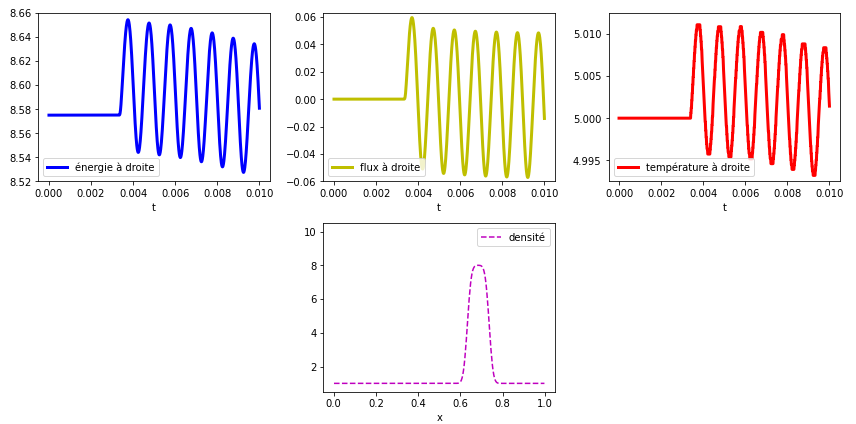
\includegraphics[width=.6\linewidth]{EntreeSortie1D} 
\decoRule
\caption[EntreeSortie1D]{Visualisation d'une entree (en haut) et d'une sortie (en bas) en 1D. Seul le signal sur la droite est utilise. Les 3 canaux E, F et T sont representes ici.}
\label{fig:EntreeSortie1D}
\end{figure}

En 1D, les entrees ne sont constituees que du signal recuperer sur le bord droit du domaine. La forme d'une example en presentee a la figure \ref{fig:Entrees1D}.

\begin{figure}[!h]
\centering
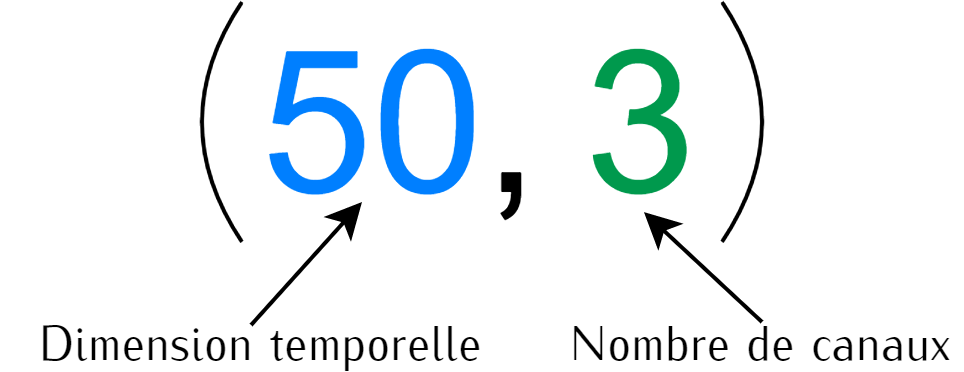
\includegraphics[width=.4\linewidth]{Entrees1D} 
\decoRule
\caption[Entrees1D]{Forme d'une entree en 1D. La dimension spatialle a ete reechantillonne de 907 a 50 iterations. Les 3 canaux designent les signaux E, F et T.}
\label{fig:Entrees1D}
\end{figure}

\subsection{En 2D}
Une entree 2D contient considerableme plus d'informatiosn. Les 3 signaux E, F et T sur les 4 bords y sont inclus. On y inclu aussi un signal correpondant a l'une des quatre positions de la source dans chacun de ces cas. En effet, une entree correspond a 4 simulations effectuees chacune avec la source a une position differente comme on peut le voire a la figure . Comparer a la 1D, il faut rajouter l'ordonnee du saut de densite pour obtenir la densite.

\begin{figure}[!h]
\centering
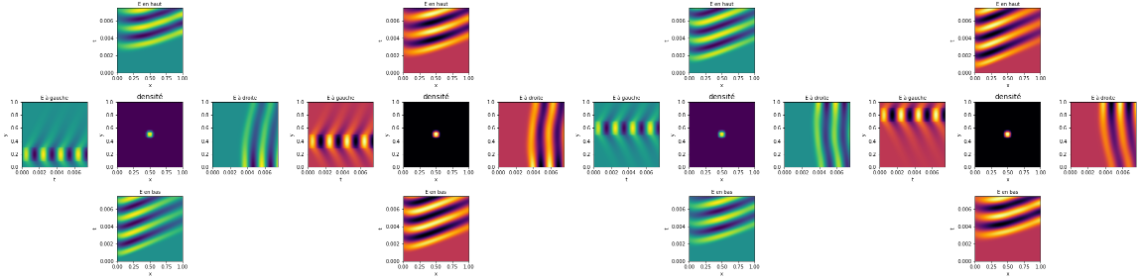
\includegraphics[width=.95\linewidth]{EntreeSortie2D} 
\decoRule
\caption[EntreeSortie2D]{Visualisation d'une entree (aux alentours des quatre images) et d'une sortie (aux mileiux) en 2D. On peut voire les postions des 4 sources utilisees a tour de role pour former une seule entree. Ici n'est representee que l'energie (qui constitue 1/3 des canaux) sur les 4 bords. Les images des densites presentee ci-contre ont ete obtenue par interpolation bilineaires d'une image initiale (28x28) moins fine.}
\label{fig:EntreeSortie2D}
\end{figure}


La forme d'une entree est representee a la figure \ref{fig:Entrees2D}. Des jeux de donnes complets 1D/2D ont ete sauvegardee et les details pour els recuperer et les traiter sont donnes en Anexe \ref{AppendixB}.

\begin{figure}[!h]
\centering
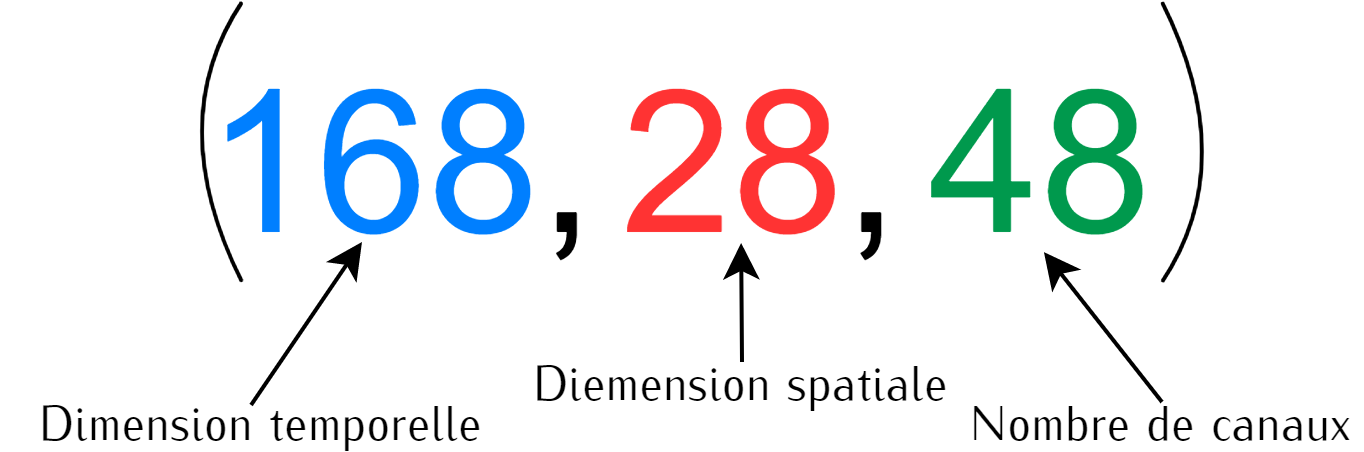
\includegraphics[width=.5\linewidth]{Entrees2D} 
\decoRule
\caption[Entrees2D]{Forme d'une entree en 2D. Contrairement a la 1D, il faut tenir compte de la dimention spatiale qui correspond au nombre de mailles sur chaque bords du domaine (N=M=28). Le nombre de canaux augmente donc considerablement. On passe a 48 car il faut tenir compte des 3 canaux originaux (E, F, et T), ensuite de chacun de 4 bords du domaine, et enfin des 4 positions de la source.}
\label{fig:Entrees2D}
\end{figure}

%----------------------------------------------------------------------------------------

\section{Architecture generale}

Un reseau de neuronnes artificel \footnote{nous y fereons reference dans la suite juste par reseau de neurones} est un systeme computationnel base sur le reseau de neuronnes biologique. L'apprentissage profond\footnote{definition du nombre de couche} permet de resoudre des problemes en Machine Learning\footnote{definition} que les methodes telles que la regression ineaire, etc.. ne peuvent pas. Il reussit cela en introduisant des representations des donnes qui s'exprimes sous forme d'autres representations, plus simples cette fois. Les reseaux profonds en aval\footnote{en oposition a un reseau de neurones recurrent qui reutilisent els resultats des model pour s'ameliorer} (ou MLP) consitituent l'exemples typique en apprentissage profond. Il s'agit juste d'une fonction (composition de differentes fonctions) faisant correspondre une serie d'entree a une serie de sortie $f^{-1} = composition de f1, f2, etc.$.

Un MLP est constitue de plusieurs couche (assimilables aux fonction f1, f2, .. precedentes) apprenant chacune un aspect particulier des donnnees (voir figure \ref{fig:MLP}. On distingue une couche d'entree, une ou pleusieurs couches cachees, et une coche de sortie).


\begin{figure}[!h]
\centering
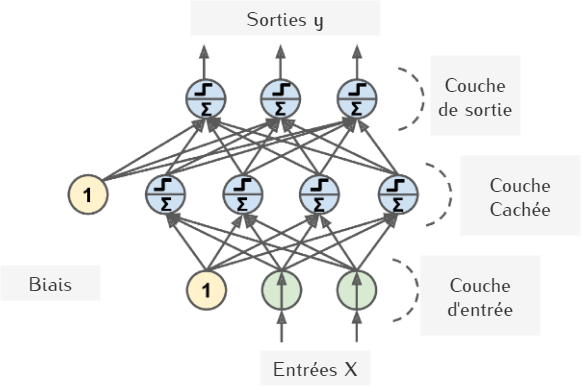
\includegraphics[width=.6\linewidth]{MLP} 
\decoRule
\caption[MLP]{Illustration d'un MLP avec une couche dense comme couche cachee. Le noombre de couche cachee peut etre elevee ce qui conduit aux reseaux de neurones profonds. Le 1 represente le biais \parencite[286]{Reference8}.}
\label{fig:MLP}
\end{figure}

Les reseaux de neurones convolutifs sont une forme de MLP spcialises dans le traitement des donnes qui ont une form de grille. Par exemple des series en temps qui peuvent etres vues comme des grilles 1D (l'axe de temps) prenant des donnes (vecteur de donnees) a interval de temps regulier \parencite{Reference5}. Ils sont donc particulieremt adaptes a la reconstruction de la densite partant des signaux temporels E, F, et T. L'archiytecture de base a ete proposee par M. Vigon. Nous utilisetons deux variantes: DRNN \footnote{Density Reconstruction Neural Network} 1 (figure \ref{fig:DRNN1}) et DRNN 2 (figure \ref{fig:DRNN2}).  Les architectures seront implemntee sous la librarie de machine leanring Keras (avec Tensorflow backend) Les differentes couches presentes seront detailles dans la suite. Nous indiquerons aussi en quoi elles sont importantes pour notre apprentissage.

% \begin{figure}[!h]
% \centering
% 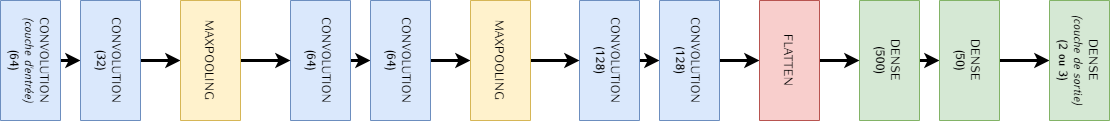
\includegraphics[width=.95\linewidth]{DRNN1} 
% \decoRule
% \caption[DRNN1]{Premeire architecture (nommee DRNN 1). Le nombre de neurnoes de la couche de sortie depend qu'on soit en 1D ou en 2D. Ce modlee contient pas des couche de Pooling\footnote{les details concernant le pooling seront donnes plus tard}. Le nombre de neurones utilises pour chaque couches est indiques entre parentheses}
% \label{fig:DRNN1}
% \end{figure}
% 
% \begin{figure}[!h] 
% \centering
% 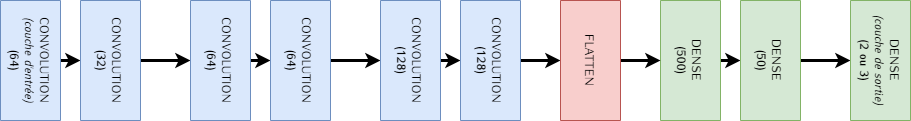
\includegraphics[width=.95\linewidth]{DRNN2} 
% \decoRule
% \caption[DRNN2]{Deuxieme architecture utilisee (nommee DRNN 2). Ce modlee ne contient pas de couches de Pooling}
% \label{fig:DRNN2}
% \end{figure}

\newpage
\begin{figure}[!ht]
   \begin{minipage}{0.6\textwidth}
     \centering
     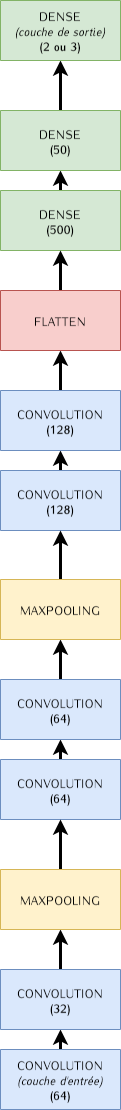
\includegraphics[width=.2\linewidth]{DRNN1ROT}
     \decoRule
     \caption[DRNN1]{Premeire architecture (nommee DRNN 1 ). Le nombre de neurones utilises pour     
     chaque couches est indiques entre parentheses. Le nombre de neurnoes de la couche de sortie 
     depend qu'on soit en 1D ou en 2D.}
     \label{fig:DRNN1}
   \end{minipage}\hfill
   \begin{minipage}{0.4\textwidth}
     \centering
     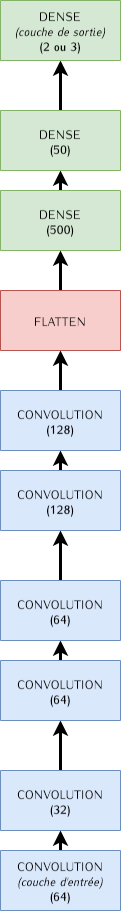
\includegraphics[width=.3\linewidth]{DRNN2ROT}
     \decoRule
     \caption[DRNN2]{Deuxieme architecture utilisee (nommee DRNN 2). Ce modlee ne contient pas de 
     couches de Pooling \footnotemark }
     \label{fig:DRNN2}
   \end{minipage}
\end{figure}
\footnotetext[6]{Les details concernant l'operation de "pooling" seront donnes a la section \ref{subsec:MaxPoling}}

% \begin{figure}[!ht]
% \begin{subfigure}{.6\textwidth}
%   \centering
%   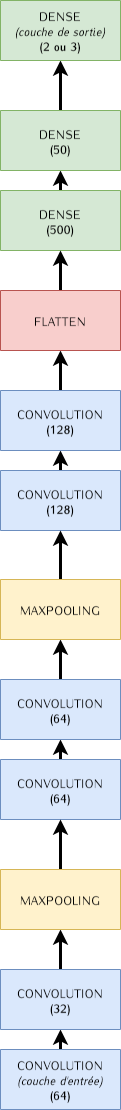
\includegraphics[width=.2\linewidth]{DRNN1ROT}  
%   \caption[DRNN1]{CPremeire architecture (nommee DRNN 1 ). Le nombre de neurones utilises pour     
%      chaque couches est indiques entre parentheses. Le nombre de neurnoes de la couche de sortie 
%      depend qu'on soit en 1D ou en 2D.}
%   \label{Fig:DRNN1}
% \end{subfigure}
% \begin{subfigure}{.4\textwidth}
%   \centering
%   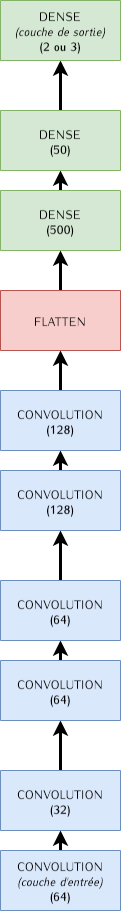
\includegraphics[width=.3\linewidth]{DRNN2ROT}  
%   \caption[Conv2D]{Deuxieme architecture utilisee (nommee DRNN 2). Ce modlee ne contient pas de 
%      couches de Pooling \footnote{Les details concernant le pooling seront donnes a la section \ref{subsec:MaxPoling}}}
%   \label{Fig:DRNN2}
% \end{subfigure}
% \label{Fig:DRNN}
% 
% \centering
% \decoRule
% \caption[DRNN]{Differents modeles de CNN utilises}
% \end{figure}
% 

----------------------------------------------------------------------------------------

\section{Les couches utilisées}

\subsection{Les couches de convolution}
la convolution est l'operation fondamentale d'un CNN. Il s'agit d'une operation lineaire qui combine deux signaux pour en extraire un troisieme. En general, une operation de convolution se definit par la formule suivante (i est le ssignal d'entree et k est le noyau de la convolution)
$$ s(t) = (i * k)(t) = \int i(x)k(t-x) \, dx $$

En pratique, les signaux temporels ne sont pas continus, ils sont discretises par interval de temps $\Delta t$. Dans ce contexte, la convolution 1D se definit par la formule:
\begin{equation}
 s(t) = \sum_{x=-\infty}^{\infty} i(x)k(t-x)
 \label{eqn:Conv1D}
\end{equation}

Cette formule doit aussi etre adaptee en 2D vu que nos inputs sont 2D. La formule devient donc:
\begin{equation}
 S(i,j) = (I * K)(i,j) = \sum_{m}\sum_{n} I(m,n)K(i-m,j-n)
 \label{eqn:Conv2D}
\end{equation}

L'operation de convolution est commutative grace a l'inversion du noyaux relativement au siganal d'entree. Cette propriete, bien qu'importante d'un point de vu therique, ne prensente pas d'avantages majeure du point de vu computationnel. C'est la raison pour laquelle on dispose de l'operation de cross-correlation qui est convolution sans inversion du noyau. En 2D elle se presente comme ceci:
\begin{equation}
 S(i,j) = (I * K)(i,j) = \sum_{m}\sum_{n} I(i+m,j+n)K(m,n)
 \label{eqn:Corr2D}
\end{equation}

On remarque aussi que le parcours des indices se fait suivant l'input. Il se trouve que c'est plus direct et rapide ainsi, parcequ'il y a moins de varaition dans la plage de valeurs valides pour $n$ et $m$. 

Plueieurs libraries de machine leanring implementent la cross-corelation mais l'appellent convolution. C'est le cas de Keras lorsqu'elle utilise le backend Tensorflow \footnote{Lorsqu'on utilise Theano, les convolutions sont effectivement des convolution comme definie en \ref{eqn:Conv1D} et \ref{eqn:Conv2D}} \parencite{Reference6}.
% 
% \begin{figure}[!h]
%     \subfloat[Convolution 1D]{
%    \begin{minipage}{0.5\textwidth}
%      \centering
%      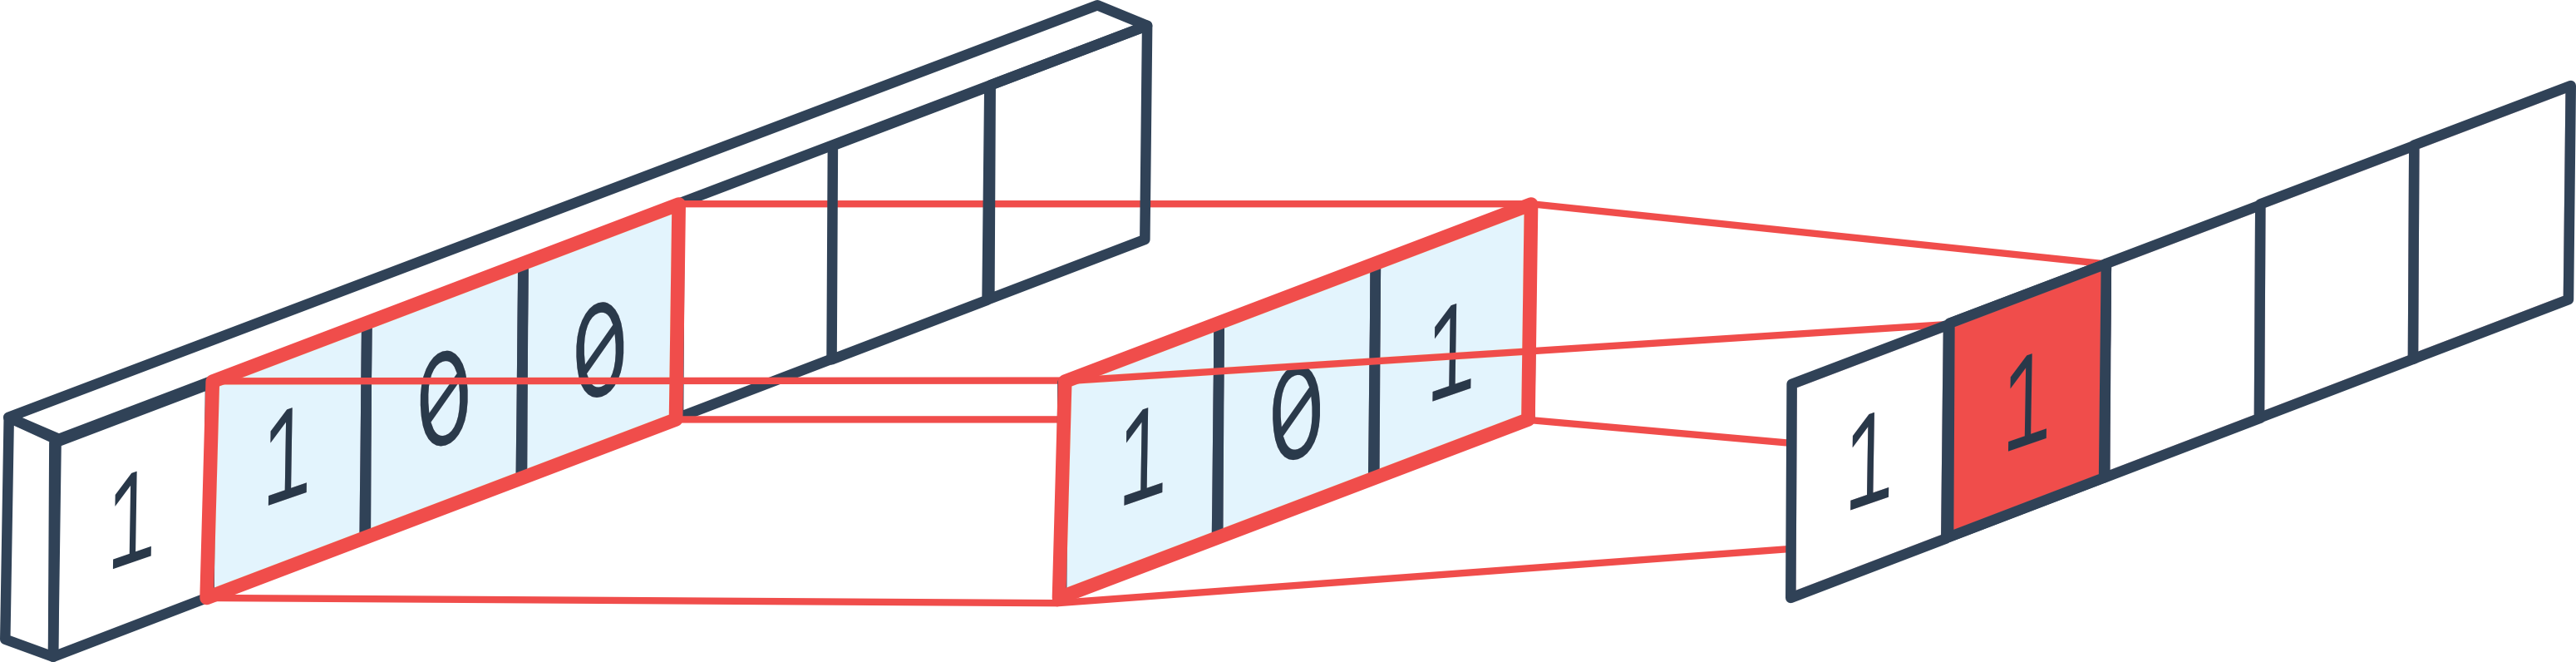
\includegraphics[width=.95\linewidth]{Conv1D}
%    \end{minipage}}
%    \hfill
%    \subfloat[Convolution 2D]{
%    \begin{minipage}{0.5\textwidth}
%      \centering
%      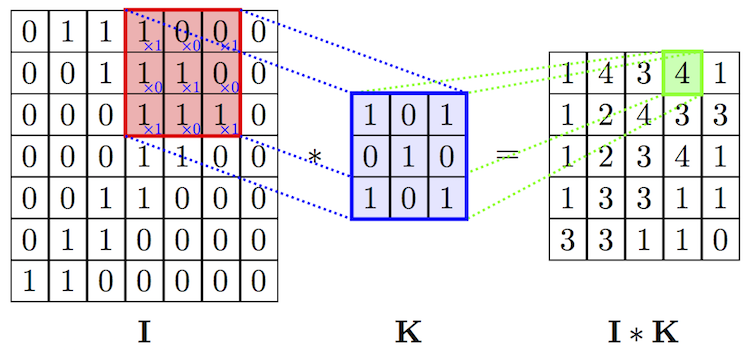
\includegraphics[width=.95\linewidth]{Conv2D}
%    \end{minipage}}
%    \label{Fig:Conv1D2D}
% 
%    \centering
%    \decoRule
%    \caption[Conv2D]{Illustration d'une convolution (cros-corelation) 1D/2D en mode "valide" (aucun padding de 0 ne sera ajoute et la sortie S aura une taille inferieure a l'entree I). La taille du noyaux que nous utiliserons sera de 3 (1D) et (6,2) (2D) . Un autre paramtre important pour reduire la taille de la sortie est le "stride", il s'agit de l'ecart entre deux applications du noyaux de convolution K. Nous le prenons egale a 1 (1D) et (1,1) (2D) de facon a couvrir tous les indices valides de l'entree I.}
% \end{figure}


\begin{figure}[!h]
\begin{subfigure}{.5\textwidth}
  \centering
  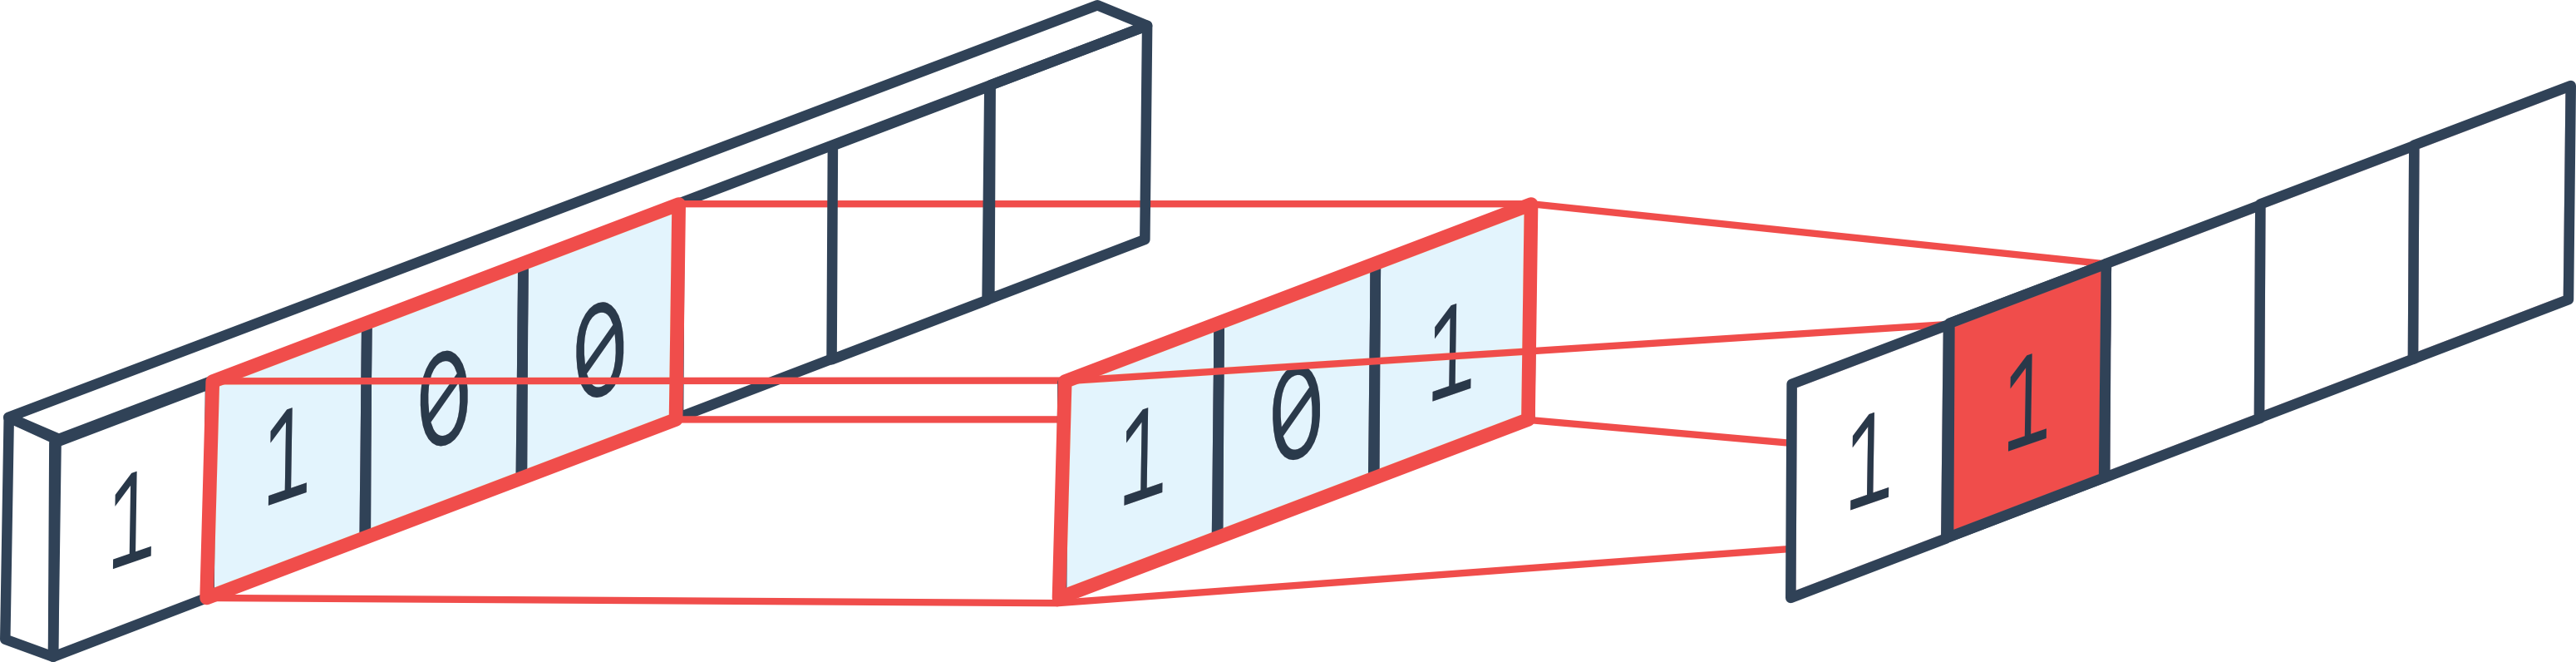
\includegraphics[width=.95\linewidth]{Conv1D}  
  \caption[Conv1D]{Convolution 1D \parencite{Reference10}}
\end{subfigure}
\begin{subfigure}{.5\textwidth}
  \centering
  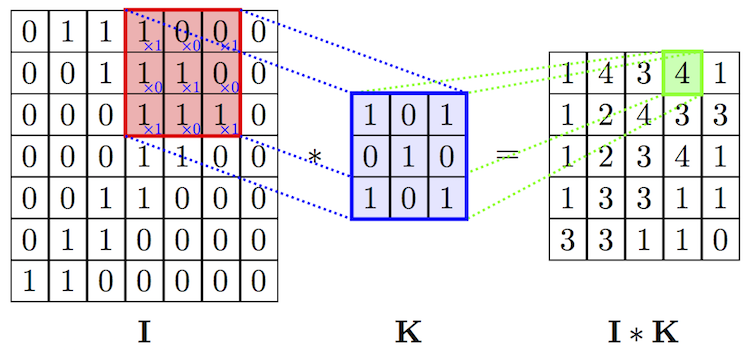
\includegraphics[width=.95\linewidth]{Conv2D}  
  \caption[Conv2D]{Convolution 2D \parencite{Reference11}}
\end{subfigure}
\label{fig:Conv1D2D}

\centering
\decoRule
\caption[Convolution1D2D]{Illustration d'une convolution (cros-corelation) 1D/2D en mode "valide" (aucun padding de 0 ne sera ajoute et la sortie S aura une taille inferieure a l'entree I). La taille du noyaux que nous utiliserons sera de 3 (1D) et (6,2) (2D) . Un autre paramtre important pour reduire la taille de la sortie est le "stride", il s'agit de l'ecart entre deux applications du noyaux de convolution K. Nous le prenons egale a 1 (1D) et (1,1) (2D) de facon a couvrir tous les indices valides de l'entree I.}
\end{figure}



% 
% Les CNN apportent trois notions cles a un apprentissage:
% \begin{itemize}
%  \item l'interaction creuse: contrairemetn aux couches traditionneles, les couches de convolution utilisent des noyaux de taille condiereblemen inferieure a celle de l'input. En terme de multiplication matricielle, cela permet de faire des taches toutes aussi importantes (detection des condouts, floutage, etc..) en ne gardant que peu de parametres en memoire et augmentant l'efficacite statitique. Cela permet aussi de reduire les couts de calcul.
%  (IMAGE)
%  \item le partage des parametres: les coefficient du noyau de convolution sont reutilises a chaque endroit de la matrice d'entree, contrairement aux couches traditionnelles qui utilise generalement chaque coefficient une seule fois.
%  (IMAGE)
%  \item la representation equivariante: le partage de parametre introduit la proprite d'equivaraition par translation. SI l'entree change, la sortie change de la meme facon, et le reseau de neurones exploite cela. Par exemple, dans l'etude d'une image, il serait interressant de detecter les contour dans la premiere couche du reseau,vu que ces meme contour sont suceptibles de reaparatire dans la suite. (\parencite{Reference5})
% \end{itemize}


Dans les architecture de CNN typiques, la couche de convolution est generalement suivi d'une etape dite de detection. Dans cette etape, les resultas lineaires de la convolution sont passes a une fonction non lineaire auniveau d'une couche de d'activaiotn. Nous detaillerons les details de l'activation dans les sections suivantes. Apres cette etape de detection, le Pooling est generalement applique pour modifier les resulats encore plus profoncdement.

\subsection{Le MaxPoling}
\label{subsec:MaxPoling}
L'operation de Pooling permet de reduire la taille des donnees (downsampling). Une fonction de pooling tranforme les entres voisines par une fonction d'aggregation statistique. Plusieurs fonctions d'aggregations peuvent etres utlisees. Par examples, le maxpooling renvoi le maximum parmis les entrees sur un domaine (rectigne en 1D et rectangulaire en 2D). 


\begin{figure}[!h]
\begin{subfigure}{.5\textwidth}
  \centering
  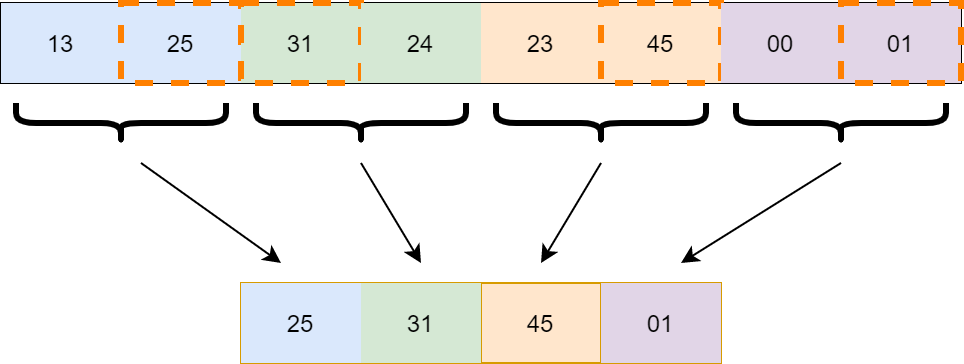
\includegraphics[width=.95\linewidth]{MaxPool1D}  
  \caption[MaxPool1D]{Maxpooling 1D}
\end{subfigure}
\begin{subfigure}{.5\textwidth}
  \centering
  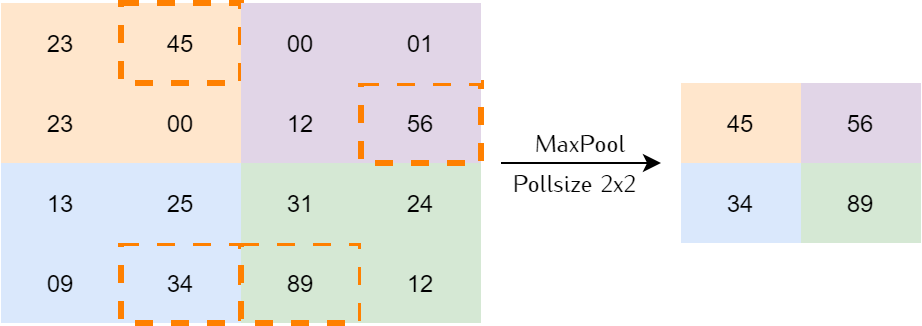
\includegraphics[width=.95\linewidth]{MaxPool2D}  
  \caption[MaxPool2D]{Maxpooling 2D}
\end{subfigure}
\label{fig:MaxPool1D2D}

\centering
\decoRule
\caption[MaxPoling]{Operatioon de maxpooling en 1D/2D avec un "pool size" de 2 (en 1D) et de 2x2 (en 2D)}
\end{figure}


En general, l'operation de pooling permet de rendre la representation approximativemtn invariante aux petite variatons dans l'input. Parlant de l'identifcation d'objects dans une image par exemple, \textit{l'invarianve par translations locales (petites tranalations) peut etre utile si on est plus interresse par la presence de l'object que par sa localisation exacte}\parencite[321ff.]{Reference5}.

Dans le probleme inverse que nous resolvons, on est aimerais non seulement detecter la presence du saut de densite, mais aussi ses coordonnes exactes. Cela nous amenera donc a considerer dans un premier temps une architecture avec pooling (figure \ref{fig:DRNN1}), et dans un dexieme temps, sans Pooling (figure \ref{fig:DRNN2}).
 
\subsection{Flatten}
L'operation d;applattissage permet de transformer les donnees en quittant de la forme tensorielle (2D avec plusieurs canaux) a une forme vectorielle. Il s'agit en realite d'une etape de preparation a une couche complement connectee.

\begin{figure}[!h] 
\centering
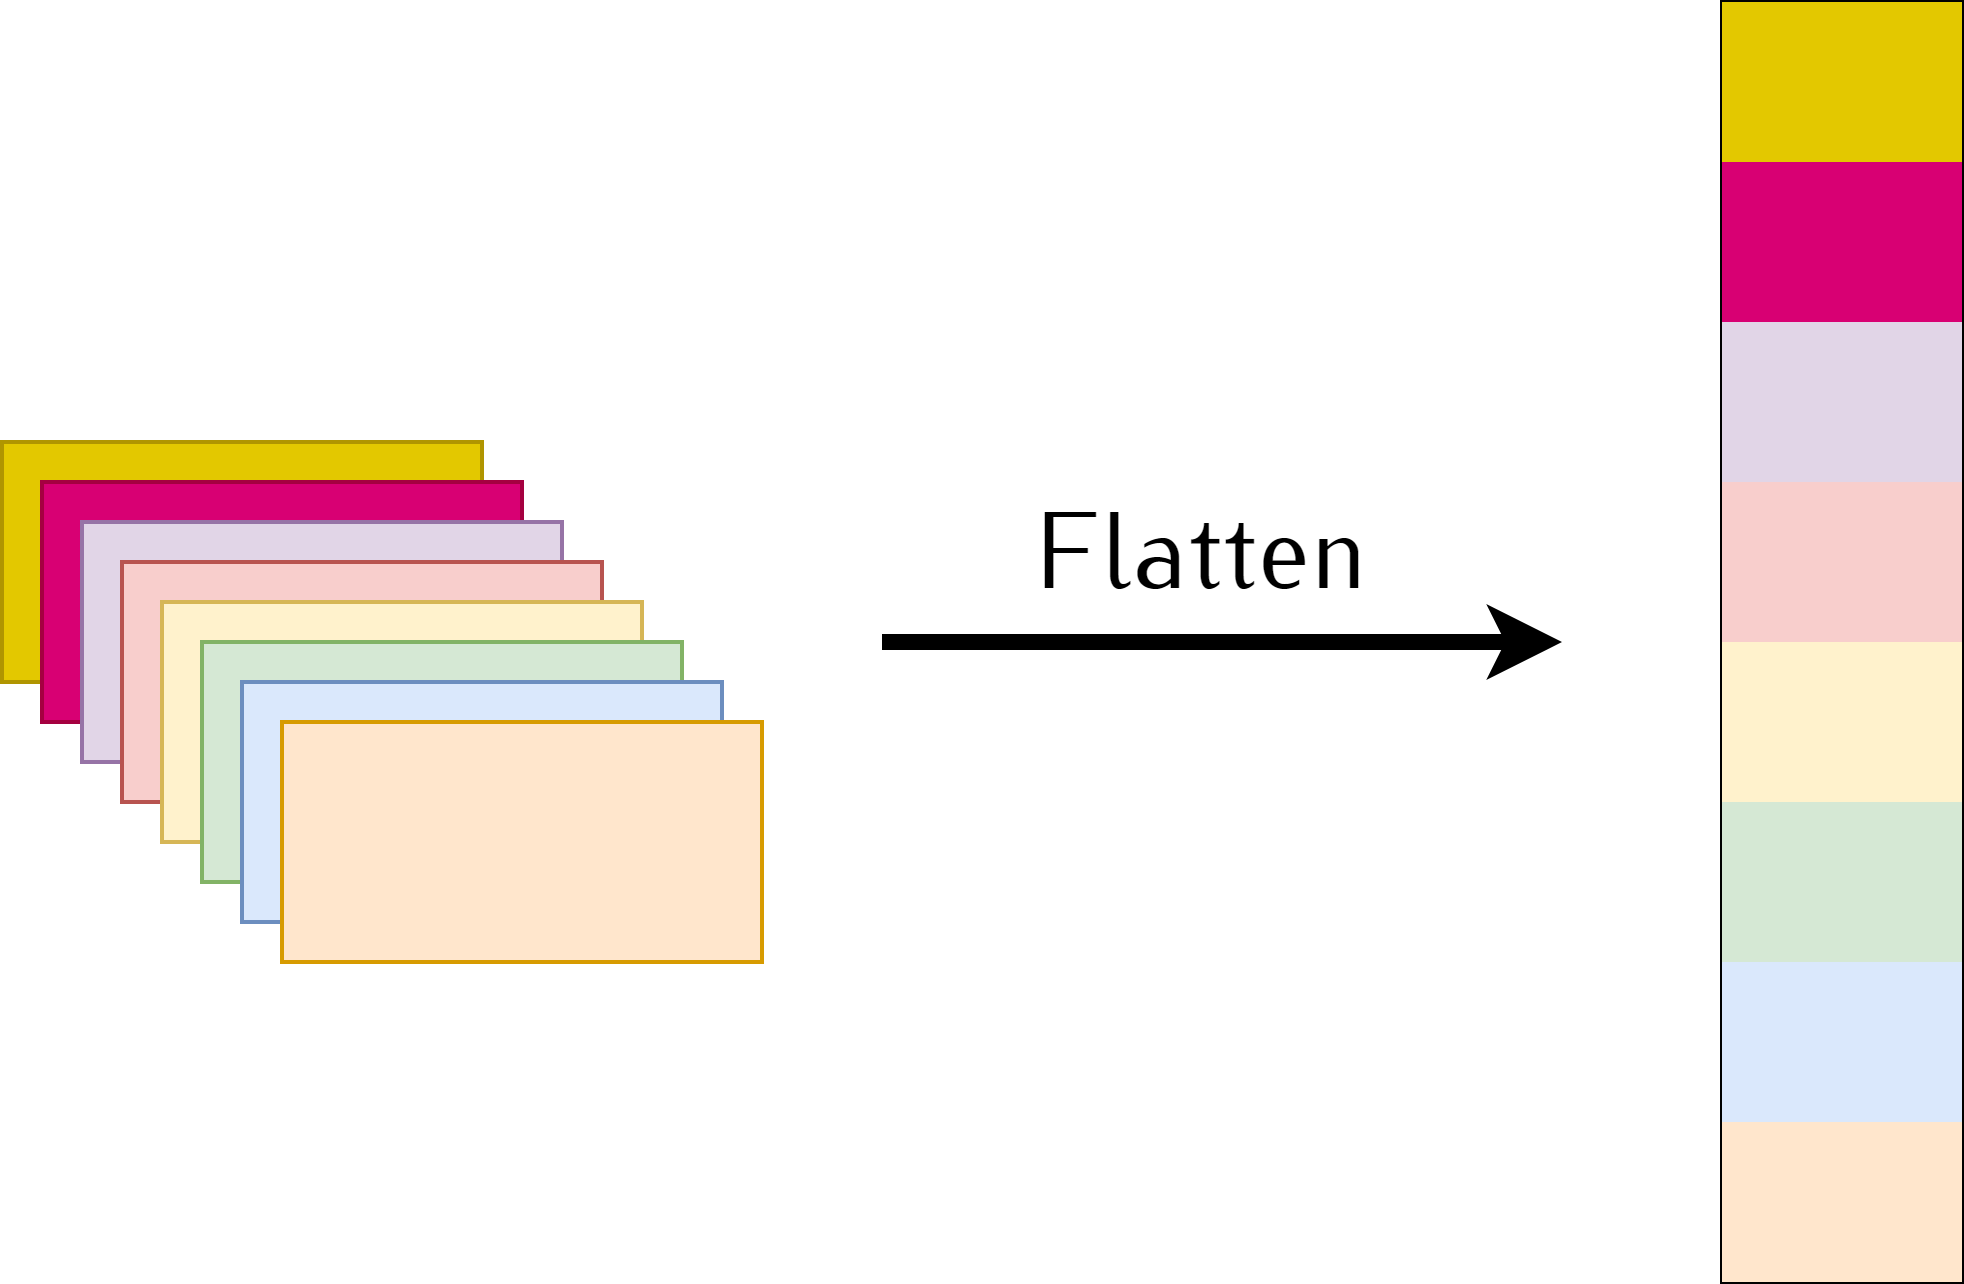
\includegraphics[width=.5\linewidth]{Flatten}
\decoRule
\caption[Flatten]{Illustration d'une operation de flatten). Qu'on soit en 1D ou en 2D, le flatten assure que la sortie est un vecteur sur lequel une couhe Dense peut operer.}
\label{fig:Flatten}
\end{figure} 

\subsection{Les couches denses}
Dans cette couche, tous les neurones sont connectes a tous les neurones de la couche precedente. Une couche dense prend les resultats d'une convolution/pooling et en resort des poinds. Les couches de convolution ayant apris des aspects particuliers des donnees, la couche est un moyen facile d'apprndre des combinaisons non lineaires de ces dernieres.

Si $f_2$ designe la fonction representant une couche dense. l'operation efffectuee est la suivante: $f_2=\phi(XW+b)$, ou $X$ represente les entrees de la couche, $b$ le bias , $W$ la matrice des poinds (une ligne par neurone d'entree et une colone par neurone de cette couche, excepte ceux du biais), et $\phi$ designe la fonction d'activation que nous detaillerons plus tard. \parencite[286]{Reference8}

\begin{figure}[!h] 
\centering
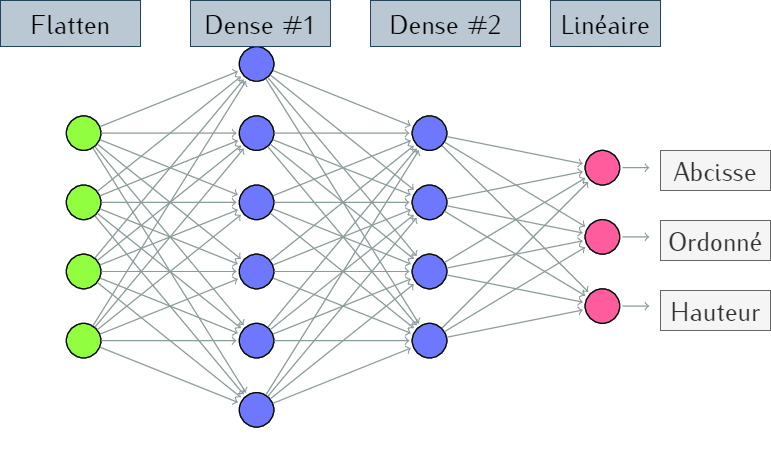
\includegraphics[width=.5\linewidth]{Dense} 
\decoRule
\caption[Dense]{Serie de 3 couches denses "fully connected". La couche (en vert) represent le resultat de l'opeation de Flatten. L'utilisation des couches denses constitue la derniere etape des reseax en figures \ref{fig:DRNN1} et \ref{fig:DRNN2}(Image adaptee de \parencite{Reference9})}
\label{fig:Dense}
\end{figure}

%----------------------------------------------------------------------------------------

\section{Configurations de l'entrainement sous Keras}
Keras proposent une multitude d'otions et d'hyperparatres pour tuner le modele. Les plus importants sont detailles dans les sections suivantes.

\subsection{Les hyper-parametres}

\subsubsection{L'optimiseur}
L'optimization est une methode d'acceleration de l'entrainement. L'optimiseur Adam\footnote{Adaptative moment estimation} combine les proprietes de deux autres algorithmes d'entrainement (AdaGrad et RMSProp).

\subsubsection{Activation RELU}
La fonction d'activation introduit une non-linearite entre les couche. L'avatage majeure de l'activation ReLU\footnote{Rectified Linear Unit} par rapport aux autres fonctions d;activation c'est qu'il n'active pas tous les neurones en meme temps. D'un pooint de vue computationel, elle est tres eficace tout en produidant des resulats satisfaisants.

\subsubsection{le taux d'apprentissage}
Il s'agit du parametre le plus influant pour notre apprentissage. Il controle a quelle vitesse le modele \footnote{les poids des neurones sont initialises de facon aleatoire} s'adapte au probleme en determinant de quelle quantite les poids des neurones seront mis a jour apres l'agorithme de backpropagation. S'il est tres eleve, il raoidement conduire a solution non optimale; s'il est tres faible, le modele peut reste fige (il fadra alors un nombre eleve d'epoques pour le debloquer).

Avec un taux d'apprentissage egale a 1e-4, nous n'avons ete capable que de detecter la hauteur du crenau en 1D; et une reduction supplementaire entraine la divergence du modele. En 2D, il a fallu descendre jusqua 1e-5 pour determiner avec precision l'abcisse, l'ordonne, et la hauteur du crenau.

\subsubsection{le batch size}
Il s'agit de la taille de chauque paquet de donnnes \footnote{nombre d'instaces d;entrainement selectiones aleatoiremetn} passes au modele durant un epoque. Un batch size faible apporte du bruit au modele vu qu'une partie aleatoire des donnes est tulisee pour mettre ajour les poids des neurones. Ceci permet une meilleure generalisation du modele tout en permettant une limiter la quantite de donnees chargee dans la RAM a chaque epoque.

% 
% \subsubsection{le coefficient de reglarisation L2}
% Le penalisation permet d;eviter le surapprentissage. Sous Keras, on peut soit penaliser les poids d'une couche (kernel optimizer), ou bien penaliser les resultats de la fonction d'activation de cette couche (activity optimizer). la deuxieme option a offert les meilleures resultats, c'est pourquoi l'avons appliquee a nos deux couches de neuronnes denses  de nos modeles avec un coefficient de 1e-5.
% 

\subsubsection{Early stopping}
La technique d'early sera notre moyen primaire de lutte contre le sur-appretisage. Pour l'implementer de facon efficace sous Keras, il nous faut une \verb|patience|. Il s'agit du nombre d'epoques a attendre avant d'areter d'areter l'apprentissage de facon precosse. Nous arreterons nos entrainement des que le score R2 (voir paragraphe \ref{subsub:R2}) sur le jeu de validation n'aura pas augmente pendant 10 epoques. 

\subsection{Les metriques}

\subsubsection{Loss MSE}
Pendant la generation des donnees, on a pris soin de pas introduire de donnes aberantes. La MSE qui est plus elevee sur les valeurs aberantes que la MAE est dont plus adaptee ici. Si les $\hat{y}_i$ designent les predictions et $y_i$ les veritables cibles (valeurs observees), la MSE se definit par:
\begin{equation}
 MSE = \frac{1}{n} \sum_{i=1}^{n} \left( y_i - \hat{y}_i \right)^2
 \label{eqn:MSE}
\end{equation}

\subsubsection{Coefficient de determination R2}
\label{subsub:R2}
Le Coefficient de determination R2 est tres important en statistique. On peut l'obtenir par la formule:
\begin{align}
 R^2 = 1 - \frac{SS_{res}}{SS_{tot}}
 \label{eqn:R2}
\end{align}
Avec
\begin{align*}
 \quad SS_{res} =  \sum_{i=1}^{n} \left( y_i - \hat{y}_i \right)^2 \quad \text{et} \quad SS_{tot} =  \sum_{i=1}^{n} \left( y_i - \bar{y} \right)^2 
\end{align*}
Ou $ \bar{y} = \sum_{i=1}^{n} y_i $ represente la moyenne des valeurs observees.

On peut remarquer que:
\begin{itemize}
 \item Si le modele predit les valeurs attendues (observees), le score R2 vaut 1. 
 \item SI le modele predit toujours la valeur moyenne $\bar{y}$, le score R2 vaut 0
 \item Si les predictions sont pires que la moyenne, le score R2 est negatif
\end{itemize}

En generalOn voit que si les predictions et les valeurs observees sont tres correles (sans etre egaux), on aura un score R2 ce qui n'est pas carateritique des resultats. En effet, pour des taches de regression il se definit comme etant le caree du coefficient de correlation entre les valeurs predites et les valeurs observees.

Dans la suite de ce rapport, le score R2 sera presente sous forme de pourcentage. 

\subsubsection{Un score personalise}
On definit donc un nouveau score particulieremtn adapte a nos donnees. On decalre qu'une prediction est correcte si elle est suffisament proche du label:
\begin{itemize}
 \item au dizième près pour la position (suivant x ou y) car le domaine de d'etude est $[0,1] \times [0,1]$
 \item à l'unité près pour la hauteur car les hauteurs observees sont comprises entre 0 et 10
\end{itemize}

Le score personalise est un score severe (pourcentage de prediction correctes) qui qui recompense les prediction qui sont a la fois precisent en hauteurs et en position. La prediction de la position etant le probleme majeure auquel nous avons fait face, il cause generalement des valeurs faibles pour le score personalise.

%----------------------------------------------------------------------------------------

\section{Resultats}

Nous resumons la sections precedentes en specifiant les paramtres (et leurs noms) utilises pour entrainer le modele sous Keras.

\begin{table}[h!]
\caption{Liste des parametres majeurs utilises pour l'entrainement. L'activation relu est utilisee sur les couches cachees et "linear" sur la couche de sortie}
\label{tab:Parametres}
\centering
\begin{tabular}{l l l}
\toprule
\tabhead{Parametre} & \tabhead{Definition} & \tabhead{Valeur 1D / 2D} \\
\midrule
\verb|learning_rate| & taux d'appentissage & 1e-4 / 1e-5\\
\verb|batch_size| & taille d'un batch a chaque epoque  & 32\\
\verb|optimizer| & algorithme d'optimisation & Adam\\
\verb|activation| & type de fonction d'activation  & "relu" ou "linear"\\
\verb|patience| & patience pour l'\verb|early_stopping| & 10\\
\verb|epochs| & nombre d'epoques & 100\\
\verb|kernel_size| & taille du noyau de convolution & 3 / (6,2)\\
\bottomrule\\
\end{tabular}
\end{table}


Nous avons entraine les architectures en 1D (fig ...) et par la suite en 2D (fig ...) en ajustant les dimensions des coushes de neurones connablement.

\subsection{Régression}
% 
    \subsubsection{En 1D}
    On obtient de tres bonnes predictions sur la hateur de l'obstacle qui affecte directement l'amplitude des signaux sur le bord droit du domaine. Ce score n'est pas assez indicatif vu que les predictions sur la position du crenaux ne sont pas assez precises. Le score personalise permet de capturer ce defaut et donne environ 25\%.
    
    Le modele avec MaxPoling correspond a la figure \ref{fig:DRNN1}, et celui sans MaxPooling a la figure \ref{fig:DRNN2}.
    
    
    \begin{table}[h!]
    \caption{Resultats obtenus sur le jeur de test en 1D. Ces valeurs representent une moyenne obtenue sur plusieurs cycles d'entrainement/prediction}
    \label{tab:Tab1D}
    \centering
    \begin{tabular}{l l l}
    \toprule
    \tabhead{Score} & \tabhead{Avec MaxPooling} & \tabhead{Sans MaxPooling} \\
    \midrule
    R2 & 99.49 \% & 99.50 \%\\
    personalise & 26.50 \% & 28.21 \%\\
    \bottomrule\\
    \end{tabular}
    \end{table}

    \begin{figure}[!h]
    \begin{subfigure}{.5\textwidth}
    \centering
    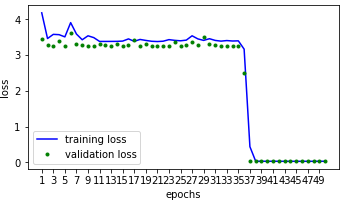
\includegraphics[width=.8\linewidth]{1DPool}  
    \caption[2DPool]{1D Avec Pooling}
    \end{subfigure}
    \begin{subfigure}{.5\textwidth}
    \centering
    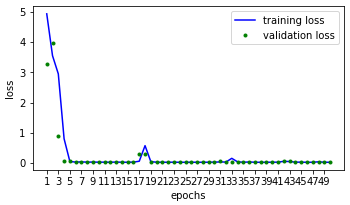
\includegraphics[width=.8\linewidth]{1DNoPool}  
    \caption[2DNoPool]{1D Sans Pooling}
    \end{subfigure}
    \label{fig:1DLoss}

    \centering
    \decoRule
    \caption[Loss 1D]{Comparaison de la vitesse de decroissiance de la loss en 1D}
    \end{figure}

    Meme si aucun n'est capable de correctement predire la position du crenau, le modele sans MaxPooling semble mieux se comporter sur ce jeu de donnees particulier. Pour les illustrations qui vont suivre, nous utilisetons donc ce dernier modele. Nous commencons par une illustration de la correlation entre les labels (valeurs observees) et les predictions (figure \ref{fig:Illustration1D}).
    
    \begin{figure}[!h]
    \begin{subfigure}{.5\textwidth}
    \centering
    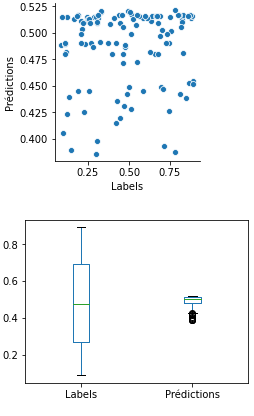
\includegraphics[width=.5\linewidth]{Position1D}  
    \caption[Pos1D]{Position}
    \end{subfigure}
    \begin{subfigure}{.5\textwidth}
    \centering
    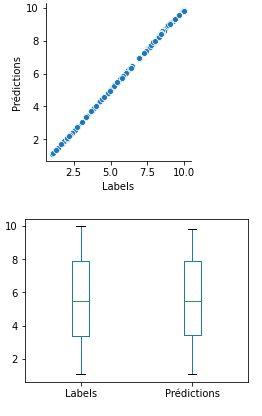
\includegraphics[width=.5\linewidth]{Hauteur1D}  
    \caption[H1D]{Hauteur}
    \end{subfigure}
    
     \centering
    \decoRule
    \caption[Illustration 1D]{Illustration de la correlation entre les labels et les predictions obtenues par le modele sans max-pooling en 1D. On peut observer l'exactitude des predictions pour la hauteur mais un echec sur la position. En effet, les predictions de la postion du crenau sont concentree autour de la moyenne 0.5}
    \label{fig:Illustration1D}
    \end{figure}

    Pour observer les meilleures et les pires predictions du modele, ils nous faut une mesure de la distance entre les predictions et les labels. On definit donc la norme ci-bas (en prenant soins de normaliser la hauteur). $$ \text{Norme} = \sqrt{\text{Position}^2 + \left( \frac{\text{Hauteur}}{10} \right)^2}$$
    
    Observons donc les meilleures predictions du modele (sans Maxpooling) (figure \ref{fig:Meilleur1D}).
    \begin{figure}[!h]
    \begin{subfigure}{.5\textwidth}
    \centering
    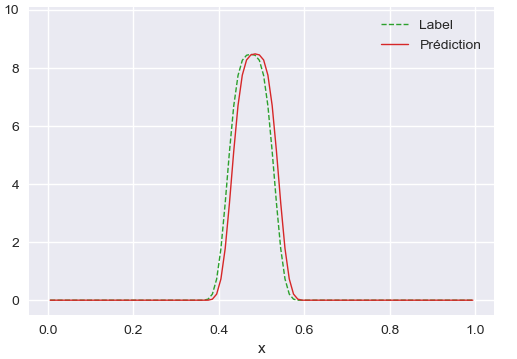
\includegraphics[width=.8\linewidth]{Meilleur1D1}  
    \caption[Meilleur1D1]{Label = [0.488 8.474] et Prediction = [0.49  8.486]}
    \end{subfigure}
    \begin{subfigure}{.5\textwidth}
    \centering
    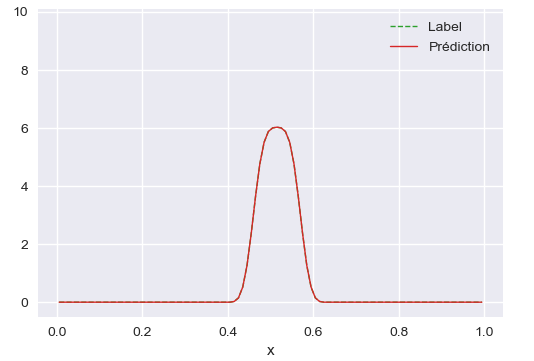
\includegraphics[width=.8\linewidth]{Meilleur1D2}  
    \caption[Meilleur1D2]{Label = [0.522 6.032]  et Prediction = [0.527 6.033]}
    \end{subfigure}
    
     \centering
    \decoRule
    \caption[Meilleur 1D]{Les meilleures predictions 1D. Il s'agit ici d'une reconstruction manuelle de la densite a partir des vecteurs presentes en (A) et (B). La premiere coordonne indique la position du saut de densite, et la deuxieme sa hauteur. On confirme que les bonnes predictions des positions sont proches du mileieu du domaine}
    \label{fig:Meilleur1D}
    \end{figure}
    
    Les pires predictions du domaine permettent de mieux illustrer les problemes rencontre avec l'apprentissage 1D (\ref{fig:Pire1D}).
    
    \begin{figure}[H]
    \begin{subfigure}{.5\textwidth}
    \centering
    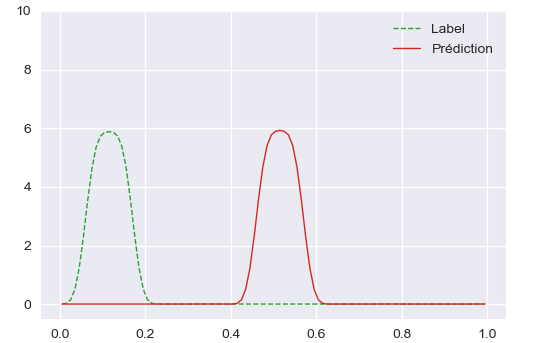
\includegraphics[width=.8\linewidth]{Pire1D1}  
    \caption[Pire1D1]{Label = [0.125 5.886] et Prediction = [0.524 5.925]}
    \end{subfigure}
    \begin{subfigure}{.5\textwidth}
    \centering
    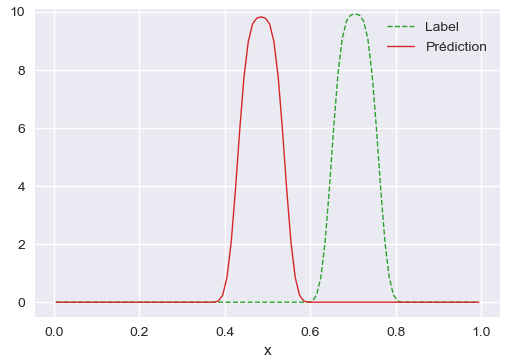
\includegraphics[width=.8\linewidth]{Pire1D2}  
    \caption[Pire1D2]{Label = [0.892 8.195]  et Prediction = [0.454 8.167]}
    \end{subfigure}

     \centering
    \decoRule
    \caption[Pire1D]{Les pires prediction du modele (sans MaxPooling) 1D. La diference se joue au niveau de la position du crenau comme indiquee a la figure \ref{fig:Illustration1D}. Les predictions les plus eloignees du mileiu sont les plus mauvaises.}
    \label{fig:Pire1D}
    \end{figure}
%     - 3eme pire prediction: label [0.302 1.066]     prediction [0.503 1.144]
    
    Le score personalise autour de 25\% indique que les prediction de la position se font quasiemnt aleatoirement. Pour remedier a ce probleme, il faut passer en 2D.  En effet, le probleme inverse est naturellement mal defini dans le sens ou plusieurs entree peuent donner la meme sortie. En 1D, on ne peut mesurer la sortie que sur un seul bord du domaine, ce qui limite beacoup notre aaprntissage.

    
    \subsubsection{En 2D}
    Comme attendu, le reseau est capable de detecter non seulment la hauteur de l'obstacle, mais aussi son abcisse et son ordonnee. Notre score personnalise nous permet de confirmer cela dans le tableau \ref{tab:Tab2D}.
    
    \begin{table}[h!]
    \caption{Resultats obtenus sur le jeur de test en 2D}
    \label{tab:Tab2D}
    \centering
    \begin{tabular}{l l l}
    \toprule
    \tabhead{Score} & \tabhead{Avec MaxPooling} & \tabhead{Sans MaxPooling} \\
    \midrule
    R2 & 94.80 \% & 98.81 \%\\
    personalise & 55.75 \% & 93.50 \%\\
    \bottomrule\\
    \end{tabular}
    \end{table}

    On constate que les modele sans l'operation de MaxPooling est globalement meileure que son homologue avec MaxPooling du a l'application de l'early stopping. La figure \ref{fig:2DLoss} permet d'observer cela a travers la vitesse de convergence du modele.
    
    \begin{figure}[!h]
    \begin{subfigure}{.5\textwidth}
    \centering
    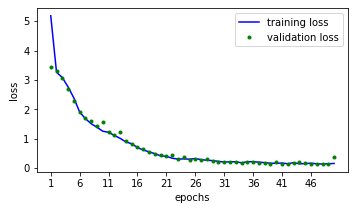
\includegraphics[width=.8\linewidth]{2DLossPool}  
    \caption[2DPool]{2D Avec Pooling}
    \end{subfigure}
    \begin{subfigure}{.5\textwidth}
    \centering
    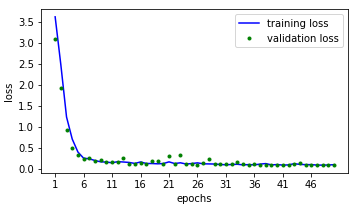
\includegraphics[width=.8\linewidth]{2DLossNoPool}  
    \caption[2DNoPool]{2D Sans Pooling}
    \end{subfigure}

    \centering
    \decoRule
    \caption[Loss en 2D]{Comparaison de la vitesse de decroissiance de la loss en 2D}
    \label{fig:2DLoss}
    \end{figure}

    COmme nous l'avons fait en 1D, Le modle sans max-pooling sera ulitlisee par la suite pour . Illustrons la correlation entre les predictions (de l'abcisse x, de l'ordonne y, et de la hauteur) et leurs labels repectifs (figure \ref{fig:Illustration2D}).
    \begin{figure}[!h]
    \begin{subfigure}{.33\textwidth}
    \centering
    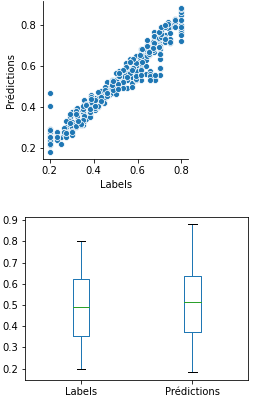
\includegraphics[width=.7\linewidth]{PositionX2D}  
    \caption[PosX2D]{Abcisse}
    \end{subfigure}
    \begin{subfigure}{.33\textwidth}
    \centering
    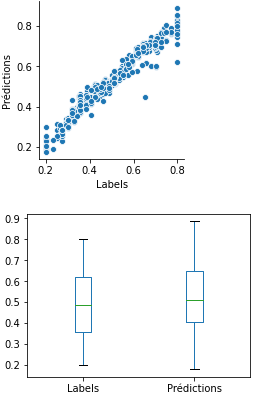
\includegraphics[width=.7\linewidth]{PositionY2D}  
    \caption[PosY2D]{Ordonee}
    \end{subfigure}
    \begin{subfigure}{.33\textwidth}
    \centering
    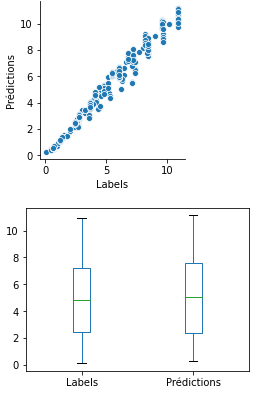
\includegraphics[width=.7\linewidth]{Hauteur2D}  
    \caption[H2D]{Hauteur}
    \end{subfigure}
    
     \centering
    \decoRule
    \caption[Illustration 2D]{Illustration de la correlation entre les labels et les predictions obtenues par le modele sans max-pooling en 2D. On peut observer que toutes les trois informations sont relativement bien correlee, d'ou le score R2 eleve (tableau \ref{tab:Tab2D}).}
    \label{fig:Illustration2D}
    \end{figure}
    
    Pour observer les meilleures et les pires predictions du modele, ils nous faut une mesure de la distance entre les predictions et les labels. On definit donc la norme ci-bas (en prenant soins de normaliser la hauteur). $$ \text{Norme} = \sqrt{\text{Abcisse}^2 + \text{Ordonee}^2 + \left( \frac{\text{Hauteur}}{10} \right)^2}$$
    
    \begin{figure}[!h]
    \begin{subfigure}{.5\textwidth}
    \centering
    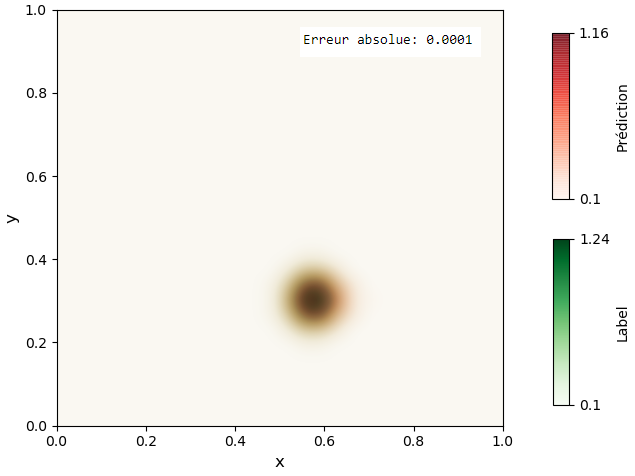
\includegraphics[width=.8\linewidth]{Meilleur2D1}  
    \caption[Meilleur2D1]{Label = [0.574 0.303 1.24 ] \\ Prediction = [0.58  0.302 1.157]}
    \end{subfigure}
    \begin{subfigure}{.5\textwidth}
    \centering
    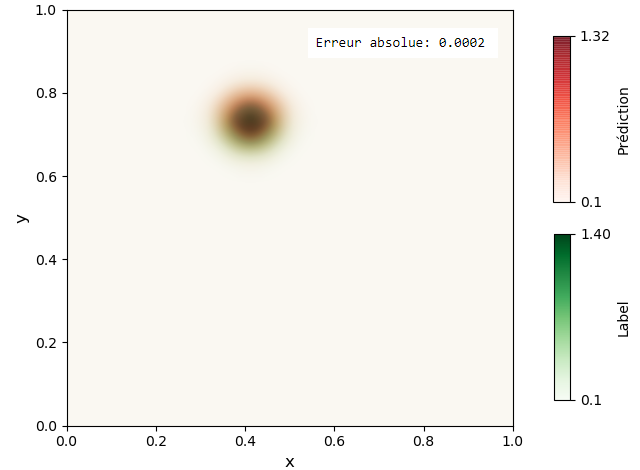
\includegraphics[width=.8\linewidth]{Meilleur2D2}  
    \caption[Meilleur2D2]{Label = [0.405 0.724 1.392]  \\  Prediction = [0.409 0.736 1.318]}
    \end{subfigure}
    
     \centering
    \decoRule
    \caption[Meilleur 2D]{Les meilleures predictions 2D. Ces images ont ete reconstruite a partir des  vecteurs "Labels" et "Prediction" issus de l'apprentissage. La premiere coordonne indique l'abcisse x du saut de densite, la deuxieme son ordonee y, et la troisieme sa hauteur. L'interpolation bicubique a ete utilise pour obtenir des images plus nettes.}
    \label{fig:Meilleur2D}
    \end{figure}

    \begin{figure}[H]
    \begin{subfigure}{.33\textwidth}
    \centering
    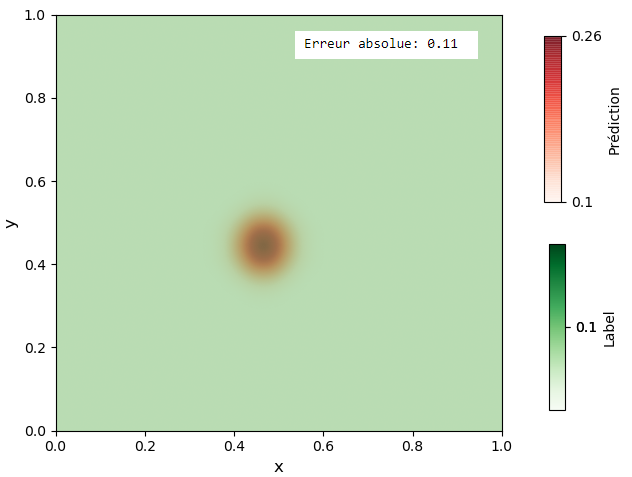
\includegraphics[width=1\linewidth]{Pire2D1}  
    \caption[Pire2D1]{Label = [0.2  0.65 0.1 ] \\ Prediction = [0.466 0.448 0.267]}
    \end{subfigure}
    \begin{subfigure}{.33\textwidth}
    \centering
    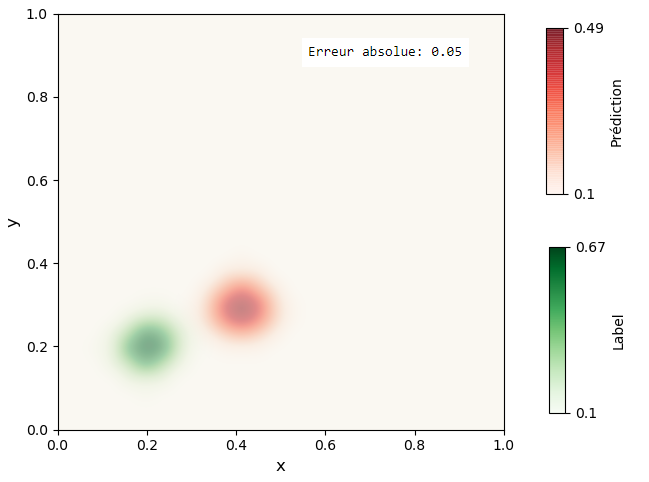
\includegraphics[width=1\linewidth]{Pire2D2}  
    \caption[Pire2D2]{Label = [0.2   0.2   0.736]  \\ Prediction = [0.407 0.298 0.494]}
    \end{subfigure}
    \begin{subfigure}{.33\textwidth}
    \centering
    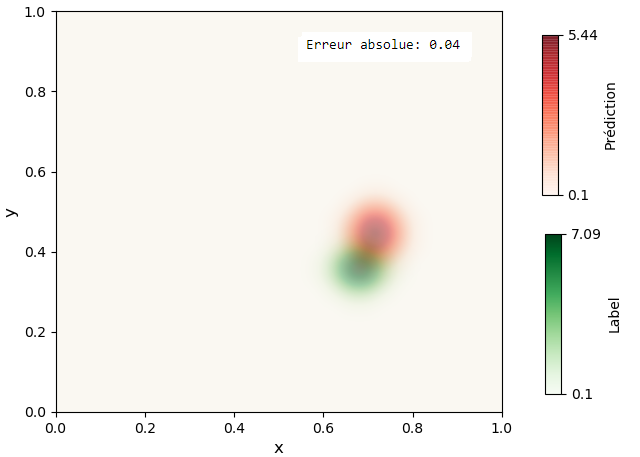
\includegraphics[width=1\linewidth]{Pire2D3}  
    \caption[Pire2D3]{Label = [0.674 0.358 7.096]  \\ Prediction = [0.712 0.449 5.462]}
    \end{subfigure}

     \centering
    \decoRule
    \caption[Pire2D]{Les pires prediction du modele 2D. Sans surprise la plus mauvaise des prediction s'obtient lorsque le crenau est absent (A). On remarque en general que les pires predictions sont faites lorsque le crenaus se situe tres proche de l'extremite (B).}
    \label{fig:Pire2D}
    \end{figure}
    
    En ce qui concerne la generalisation du modle a d'autres formes d'obstacles, je n'ai pas eu l'ocasion de comparer les modeles avec et sans max-Pooling. Le modele sans MaxPooling risque alors d'etre moins performant conformement a la theorie (voir paragraphe \ref{subsec:MaxPoling}). Sous Keras, le modele a prouver etre capable d'apprendre en continu, du moment que les entrees soient toutes normalisee et ayant la meme forme.

\subsection{Classification}
Durant le stage, il a fallu effectuer une classification mutilabel sur les donnes en 2D. QUi permet de placer l'obstacle dans une categorie definie a partir de la source. La classification petmet de detecter juste l;ordonne de l'obstacle. La structure des entrees est quasiment la meme que pour la regression, sauf qu'il manque les signaux sur la gauche (ou se trouve la source). En ce qui concerne les sorties, l'image ci-dessous decrit mieux leur structure:

\begin{figure}[!h] 
\centering
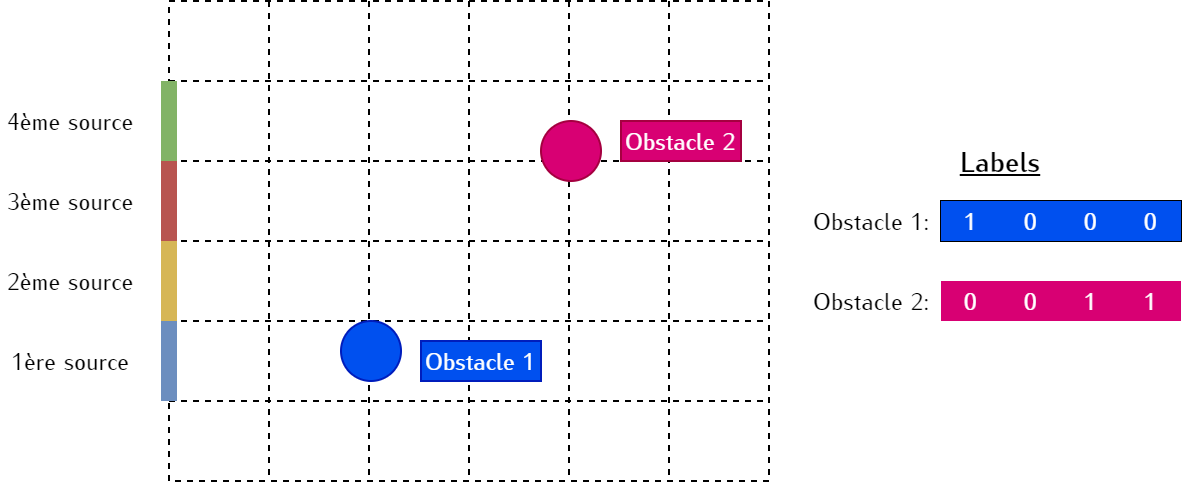
\includegraphics[width=.8\linewidth]{Classification} 
\decoRule
\caption[Classification]{Description des labels pour la classification multilabel en 2D. Un label est marque 1 si l'obstacle se touve dans le champ de la source correpondante}
\label{fig:Classification}
\end{figure}

Les donnnes utilisee pour la classification ont une shape differente des autre. On a moins d'iterations en temps (40 au lieu de 168) mais mais un maille beacoup plus fin (90x90 au lieu de 28x28). L'architecture du modle utilise ressemble celle de la regression. Une majeure difference est qu'on utilise une activation "sigmoid" a la place de l'activation "lineaire". On obtient donc en sortie des probabilites qu'il faut classer par categories. Le modele est entraine avec des hyper-parametres identiques a ceux utilisees durant les regression. Les resultats sont presentes a la table \ref{tab:Class}

\begin{table}[h!]
\caption{Resultats obtenus pour la classification en 2D. Le score severe favorise les predictions qui sont exactes au veritable sur tous les 4 colones . Le seuillage permet d'augmenter la precision des resultats en se fixant un nouveu seuil a partir duquel les interpreter les sorties du reseau de neurones. Le score de Binary Accuracy procure par keras est calcule avant seuillage.}
\label{tab:Class}
\centering
\begin{tabular}{l l l}
\toprule
\tabhead{Score} & \tabhead{Avec MaxPooling} & \tabhead{Sans MaxPooling} \\
\midrule
Binary accuracy & 75.00 \% & 98.86 \%\\
Score severe apres seillage & 27.27 \% & 95.45 \%\\
\bottomrule\\
\end{tabular}
\end{table}

\begin{figure}[!h]
\begin{subfigure}{.5\textwidth}
\centering
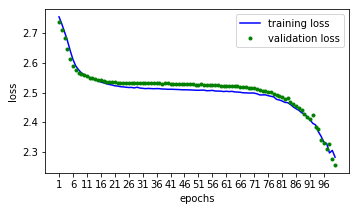
\includegraphics[width=.8\linewidth]{ClassPool}  
\caption[2DPool]{2D Avec Pooling}
\end{subfigure}
\begin{subfigure}{.5\textwidth}
\centering
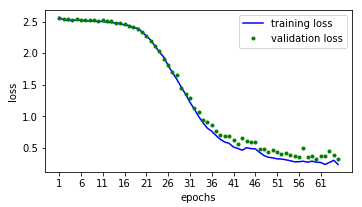
\includegraphics[width=.8\linewidth]{ClassNoPool}  
\caption[2DNoPool]{2D Sans Pooling}
\end{subfigure}

\centering
\decoRule
\caption[ClassLoss]{Comparaison de la vitesse de decroissiance de la loss (multilabel crossentropy) pour la classification en 2D}
\label{fig:ClassLoss}
\end{figure}


\begin{figure}[H] 
\centering
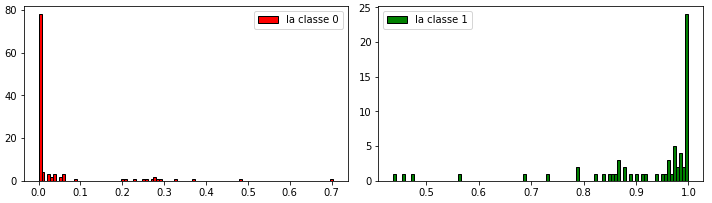
\includegraphics[width=.8\linewidth]{ClassFiabilite} 
\decoRule
\caption[ClassFiabilite]{Confiance du modele sans max-pooling en ses prediction. En rouge la classe 0 qui indique l'abscence du crenau devant la source; et en vert la classe 1. Cette figure indique que le modle se trompre rarement, ce qui confirme le resultat abtenu a la table \ref{tab:Class}.}
\label{fig:ClassFiabilite}
\end{figure}


Dans ce cas aussi, le modele sans Maxpooling seble meilleure (figures \ref{fig:ClassLoss} et \ref{fig:ClassFiabilite}). Cependant nous ne disposons pas d'axxez de donnes pour verifier celui qui se generalise mieux. Ceci etant une classifcation,  les meilleures prediction du meilleure modele sont exactement les labels attendus et les pires predictions ne varient que de peu (de 1) de leurs cibles. Il est interressnat de constater qu'il n'y a aucune prediction aberante, par exemple: un obstacle se trouve en face des sources 1 et 3 sans recontrer la source 2.

%----------------------------------------------------------------------------------------

% Chapter 5

\chapter{Bilan du stage} % 5th chapter title

\label{Chapter5} % For referencing the chapter elsewhere, use \ref{Chapter5} 

%----------------------------------------------------------------------------------------

\section{Ressources utilisées}

Les ressources utilisee durant le stage varient en nature et en fonction.

\subsection{Ecriture du Code}
\begin{itemize}
 \item VSCode: Pour l'edition du (principalemtn C++) grace a ses fonction. L'extension majeure ici est CMake.
 \item Google Colab: Facilitation de l'apprentissage sous Keras grace a ses GPU. Les libraries majeures ici sont Numpy, pandans, et Keras.
 \item Jupyter: Pour les taches en Python ne necessitant pas trop de resource (visualisation, sauvegarde en format PQT). Les librairies majeures utilisees ici sont Numpy, Pandas et Matplotlib.
 \item Kile: Pour l'ecritude du rapport en Latex
 \item Draw.io: Pour les illustrations 
\end{itemize}


\subsection{Communication}
Les communications se sont effectuees principalemtn par messagerie electronique. j'ai aussi eu l'occasion de communiquer avec les proffeseurs en presentiel a 3 reprise.

%----------------------------------------------------------------------------------------

\section{Journal de bord}

\subsection{Semaine 1 et 2}
\begin{itemize}
 \item 15 juin: Reunion de debut de Stage par Google Meet
 \item 16 juin: Demande aux professeurs de verifier un example de simulation 1D, avant de me lancer la generation des donnnees
 \item 17 juin: Remarque du problem d'apparition du crenau sur l'energie 
 \item 18 juin: Redaction d'un nouveau schema par M. Franck (pour l'etape 1) qui devrait conserver l'equilibre
 \item 22 juin: Detection de la source du probleme du crenau sur E, et redefinition des termes. 
 \item 23 juin: Confirmation de l'exactitude des simulations 1D et debut de la generation des donnes avec 500 mailles.
\item 25 juin: Demande d'aide a M. Vigon pour la configuration de la fonction d'activation de la couche de sortie
\end{itemize}


\subsection{Semaine 3 et 4}

\begin{itemize}
 \item 3 juillet: Rencontre avec M. Navoret pour discuter des avancements. Prise de connaissance de d'une des raisons potentielles du probleme de mauvaise prediction de la position du crenau sur la densite en 1D. Proposition de plusieurs solutions par M. Navoret, entre autre de partir d'un signal stationanire sinnusoidal et d'introduire l'onde a un temps t*>0.
 \item 6 juillet: Nouvelles simualtions effectues en vue d'observer la difference entre les effets de deux densites differentes. Continuation vers des nouvelles simualtiosn avec 300 mailles.
 \item 8 juillet: decroissance du taux d'apprentissage a la suggestion de M. Franck mais non amelioration des resultats d'apprentissage.
 \item 9 juillet: Passage aux reseaux convolutif grace a M. Vigon
 \item 11 juillet: Plot du debut des oscillation, des maximum, des minimum a la demande de M. Vigon, afin de mieux observer les effet de deux crenaux de densite diferents. 
\end{itemize}

\subsection{Semaine 5 et 6}

\begin{itemize}
 \item 13 juillet: Rencontre avec M. Navoret et M. Franck a la fac. Denvant la persistance du probleme de non detection de la position du crenau, l'implementation du probleme en 2D semble etre la solution approprie.
 \item 14 juillet reformulation 2D du schema de splitting et adaptation du code 1D en 2D
 \item 19 juillet: fin du codage 2D  er presentation des resultats
 \item 25 juillet: ajustemetn de la gamme de couleurs pour les visualisations et passage a la generation des donnes sur 90x90 mailles.
\end{itemize}

\subsection{Semaine 7 et 8}
\begin{itemize}
 \item 5 aout: Rencontre avec M. Franck a la fac. Proposition de solutions pour la non dectection de la position du crenau en 2D par resolution d'un systeme proche de l'eq de la chaleur, apres affichage par ligne de niveau. La possibilite d'adopter un obstacle s'etendant sur toute la verticale est envidagee. Prise de connaissance des delains pour la redaction du rapport.
 \item 6 aout: Redaction et envoi du plan du rapport de stage. 
 \item 7 sout: Proposition de reduction drasque de resolution spatiale par M. Vigonm, et proposition de nouvelles idees par M. Vigon, entre autre la consideration d'un obstacle considerableme plus opaque.
 \item 8 sout: Nouvel apprentissage avec des simplification majeures qui fonctionnne. Melioration des resultats et continuation du rapport.
\end{itemize}
%----------------------------------------------------------------------------------------

\section{Difficultés rencontrées et solutions apportées}

\subsection{Apparition d'un crenau sur E}
Au totu debut du stage, un crenau se formait puis se propageait sur l'energie E, le flux F et la temperature T. Grace a mes encadrant, ce probleme a ete resolu par rajout d'un terme au niveau de la deuxieme equation du schema de splitting.

\subsection{Detection de la position du crenau}
La detection de la position du saut de densite a ete un probleme majeure durant le stage. A la fin stage, aucune solution (si elle existe) n'a ete trouvee pour le probleme inverse en 1D. 
Cependant en 2D le probleme a ete resolu essentiellment par augmentation du nombre d'epoques et dimunution du taux d'appretissagee a 1e-5. Il est bien connu que les problemes de machine peuvent diverger si le taux d'apprentissage est trop eleve. Quand au nombre d'eqpoques, je n'en faisait pas suffisament pour voir le modele converger. Une solution bien plus rapide aurait ete d'automatiser la recherche des hyper-parametres, chose que je n'ai apprise qu'a la fin du stage.

\subsection{Gestion du temps}
La gestion du temps durant le stage n'a aps ete facile. Au moment d'imimpplementer le schema en 2D (ce qui n'etait pas initialement prevu), j'ai longement hesiter sur l'option la plus rapide. J'ai pu compter sur les conseils de M. Navoret pour surmonter cet obstacle. 

Aussi, je me suis rendu compte des delais bien en retard, j'ai du me debrouiller pour ameliorer les resultat et terminer l'apprentissage. Cela dit, je n'ai pas reussi a faire une partie essentielle qui consiste a verfier comment un modele un modele avec MaxPooling se generalise mieux qu'un modele sans.

%----------------------------------------------------------------------------------------

\section{Les apports du stage}

Ce stage a ete enrichissant pour moi sur plusieurs front:

\subsection{Experience en developpement}
J'ai gagne de l'experience en development C++ et Python, tout en me developant un portfolio. J'ai beaocup apris sur l'API de Pandas, Matplotlib, et plus important encore, celle de Keras. J'ai a present une large base de donnes de code reutilisable pour d'autres taches.

\subsection{Equations aux derivee aprtielles}
J'ai pu observer directemnt quelques astuces utilisees par mes maitres de stages pour verfier la validite de la modelisatopm d'une EDP. Pour l'equation du transfer radiatif, j'ai compris la necessite de partir d'un etat d'equilibre radiatif.

\subsection{Reseau de neurones}
Ce stage m'a permis de percevori la puissance des reseaux de neurones. J'ai appris a quel point le taux d'apprentissage est important. Comme mentionne dans le livre de reference Deep learning \textit{The learning rate is perhaps the most important hyperparameter. If you have time to tune only one hyperparameter, tune the learning rate} \parencite[417]{Reference5}. 

J'en ressort aussi avec quelques question concernant le batch size. Lors de l'apprentissage, il a fallu entrainer le modele en utlisant la methode d'augmentation du batch size pour obtenir les premiers "bons" resultats. Cette methode referencee ici (LiEN RETROUVABLE DANS LES MAIL) montre que beacoupd de questions restent a resoudre dans le domaine du deep learning.

\subsection{Experience de recherche}
En tant que premiere experience dans un environnement de recherche tel que l'UFR, j'ai pu me familirser avec le milieu. J'ai notament apris que les resultats ne doivent pas toujours etre ceux auxquels on s'attends, du moment que l'on a une explication de l'echer.

%----------------------------------------------------------------------------------------

% Chapter 6

\chapter{Conclusion} % 6th chapter title

\label{Chapter6} % For referencing the chapter elsewhere, use \ref{Chapter6} 

%----------------------------------------------------------------------------------------

Pour conclure, j’ai effectué mon stage de master 1 en tant que stagiaire en calcul scientifique/ data scientist au sein de l'UFR de mathemtiques et d'informatiques de l'Unistra. Lors de ce stage de 2 mois, j’ai pu mettre en pratique mes connaissances en developemtnt C++ et Python acquises durant ma formation en calcul scientifique et mathematiques de l'informtion. Je me suis confronte au problem inverse de reconstruction de la densite d'un domaine par un CNN apres avoir modelisaer la propagation du signal dans ce dernier en 2D.

Ce stage fut tre enrichissant pour moi car il m'a permis d'approfondir mon savoir theorique sur les la backpropagation et la descente de gradient utilises dans les reseaux de neurones malgres le fait que j'y ai passe relativemetn peu de temps. J'ai aussi gagne beacoup d'experience de development logiciel et je me suis familiarise avec l'environnement de Keras. Par contre je n'ai aps eu l'ocasion de mieux comprendre la theorie des EDP, en particulier l'intuition derriere la definition des flux numeriques dans les schema. Ce stage m’a aussi permis de comprendre le deroulement d'une activite de recherche, et a quel point une bonne organisation et un certains degre d'autonomie sont importants. Ce stage a donc confote mon projet de m'orinter vers un poste de ...

Cette experience de stage fut centree autour de la prolematique de l'apport des reseaux de neuronnes dans la resolution des problemes inverse, specialement dans la detection des tumeurs \footnote{les tumeurs sont assmilables a des crenaux, des sauts de densite, ou obstacles}. Les reseaux de neuronnes sont capables de detecter des sauts de natures bien variees, sous des conditions variees (opcites d'absoption differentes, maillage varies, etc..), tout ceci avec un cout de calcul relativement faible.

Fort de cette experience et de ses nombreux enjeux, j'aimerais beacoup par la suite, via un prochain stage,  affiner les resultats a l'aide d'un apprentissage en continue en passant a la detection de plusieurs sauts de densite par exemple. Tout ceci pourrais conduite ultimement a la creation d'un tomographe et un deploiment en milieu medical.


%----------------------------------------------------------------------------------------
%	THESIS CONTENT - APPENDICES
%----------------------------------------------------------------------------------------

\appendix % Cue to tell LaTeX that the following "chapters" are Appendices

% Include the appendices of the thesis as separate files from the Appendices folder
% Uncomment the lines as you write the Appendices


% Appendix A

\chapter{Comment reproduire les resultats?} % Main appendix title

\label{AppendixA} % For referencing this appendix elsewhere, use \ref{AppendixA}

\section{Execution du code 1D/2D}

Pour compiler le code de resolution de l'EDP, on a deux options:

\begin{itemize}
 \item Utiliser Cmake
 \item Utiliser Docker
\end{itemize}

\section{Sauvegarde des resulats}

\section{Execution des notebook et apprentissage}


% Appendix B

\chapter{Comment faire des prédictions avec ce modèle?} % Appendix B title

\label{AppendixB} % For referencing this appendix elsewhere, use \ref{AppendixA}
Pour faire des prédications, il suffit de disposer d'un jeu de données ayant la forme bien particulière décrite à l'une des figures \ref{fig:entrees1D} ou \ref{fig:entrees2D}. Il faut ensuite charger le modèle à l'aide de Keras et ensuite le compiler.

\section{Normalisation des données}
En plus d'avoir la forme appropriée, les données doivent être normalisées i.e toute les énergies doivent êtres divisées par leur maximum (en valeur absolue). Il en est de même pour le flux et la température.

\section{Chargement du modèle}
Le modèle a été sauvegardé sous la convention HDF5 de Keras. Après l'avoir chargé, il faut le compiler avec l'optimiseur Adam (et un taux d'apprentissage de \verb|1e-4| ou \verb|1e-5| suivant qu'on soit en 1D ou 2D). Pour que la compilation fonctionne, il faut impérativement inclure la fonction de calcul du sore $R^2$ indiquée ci-dessous.

\begin{verbatim}
from keras import backend as K

 def r2_score(y_true, y_pred):
    SS_res =  K.sum(K.square(y_true - y_pred), axis=-1) 
    SS_tot = K.sum(K.square(y_true - K.mean(y_true)), axis=-1)
    return 1.0 - SS_res/(SS_tot + K.epsilon())
\end{verbatim}


\section{Entrainer le modelé en continu}
Le modèle peut être entraîné en continu. Après l'avoir chargé, on peut l'apprendre à détecter d'autres formes d'obstacles sous différentes conditions. Il suffit déjà de disposer de telles données. Pour l'apprentissage en continu, on pourra utiliser la fonction \verb|train_on_batch| de Keras.


%\include{Appendices/AppendixC}

%----------------------------------------------------------------------------------------
%	BIBLIOGRAPHY
%----------------------------------------------------------------------------------------

\printbibliography[heading=bibintoc]

%----------------------------------------------------------------------------------------

\end{document}

